% Options for packages loaded elsewhere
% Options for packages loaded elsewhere
\PassOptionsToPackage{unicode}{hyperref}
\PassOptionsToPackage{hyphens}{url}
%
\documentclass[
  italian,
  letterpaper,
  paper=6in:9in,
  pagesize=pdftex,
  headinclude=on,
  footinclude=on,
  11pt]{scrbook}
\usepackage{xcolor}
\usepackage{amsmath,amssymb}
\setcounter{secnumdepth}{5}
\usepackage{iftex}
\ifPDFTeX
  \usepackage[T1]{fontenc}
  \usepackage[utf8]{inputenc}
  \usepackage{textcomp} % provide euro and other symbols
\else % if luatex or xetex
  \usepackage{unicode-math} % this also loads fontspec
  \defaultfontfeatures{Scale=MatchLowercase}
  \defaultfontfeatures[\rmfamily]{Ligatures=TeX,Scale=1}
\fi
\usepackage{lmodern}
\ifPDFTeX\else
  % xetex/luatex font selection
\fi
% Use upquote if available, for straight quotes in verbatim environments
\IfFileExists{upquote.sty}{\usepackage{upquote}}{}
\IfFileExists{microtype.sty}{% use microtype if available
  \usepackage[]{microtype}
  \UseMicrotypeSet[protrusion]{basicmath} % disable protrusion for tt fonts
}{}
\makeatletter
\@ifundefined{KOMAClassName}{% if non-KOMA class
  \IfFileExists{parskip.sty}{%
    \usepackage{parskip}
  }{% else
    \setlength{\parindent}{0pt}
    \setlength{\parskip}{6pt plus 2pt minus 1pt}}
}{% if KOMA class
  \KOMAoptions{parskip=half}}
\makeatother
% Make \paragraph and \subparagraph free-standing
\makeatletter
\ifx\paragraph\undefined\else
  \let\oldparagraph\paragraph
  \renewcommand{\paragraph}{
    \@ifstar
      \xxxParagraphStar
      \xxxParagraphNoStar
  }
  \newcommand{\xxxParagraphStar}[1]{\oldparagraph*{#1}\mbox{}}
  \newcommand{\xxxParagraphNoStar}[1]{\oldparagraph{#1}\mbox{}}
\fi
\ifx\subparagraph\undefined\else
  \let\oldsubparagraph\subparagraph
  \renewcommand{\subparagraph}{
    \@ifstar
      \xxxSubParagraphStar
      \xxxSubParagraphNoStar
  }
  \newcommand{\xxxSubParagraphStar}[1]{\oldsubparagraph*{#1}\mbox{}}
  \newcommand{\xxxSubParagraphNoStar}[1]{\oldsubparagraph{#1}\mbox{}}
\fi
\makeatother


\usepackage{longtable,booktabs,array}
\usepackage{calc} % for calculating minipage widths
% Correct order of tables after \paragraph or \subparagraph
\usepackage{etoolbox}
\makeatletter
\patchcmd\longtable{\par}{\if@noskipsec\mbox{}\fi\par}{}{}
\makeatother
% Allow footnotes in longtable head/foot
\IfFileExists{footnotehyper.sty}{\usepackage{footnotehyper}}{\usepackage{footnote}}
\makesavenoteenv{longtable}
\usepackage{graphicx}
\makeatletter
\newsavebox\pandoc@box
\newcommand*\pandocbounded[1]{% scales image to fit in text height/width
  \sbox\pandoc@box{#1}%
  \Gscale@div\@tempa{\textheight}{\dimexpr\ht\pandoc@box+\dp\pandoc@box\relax}%
  \Gscale@div\@tempb{\linewidth}{\wd\pandoc@box}%
  \ifdim\@tempb\p@<\@tempa\p@\let\@tempa\@tempb\fi% select the smaller of both
  \ifdim\@tempa\p@<\p@\scalebox{\@tempa}{\usebox\pandoc@box}%
  \else\usebox{\pandoc@box}%
  \fi%
}
% Set default figure placement to htbp
\def\fps@figure{htbp}
\makeatother



\ifLuaTeX
\usepackage[bidi=basic]{babel}
\else
\usepackage[bidi=default]{babel}
\fi
% get rid of language-specific shorthands (see #6817):
\let\LanguageShortHands\languageshorthands
\def\languageshorthands#1{}


\setlength{\emergencystretch}{3em} % prevent overfull lines

\providecommand{\tightlist}{%
  \setlength{\itemsep}{0pt}\setlength{\parskip}{0pt}}



 


\KOMAoptions{DIV=12, BCOR=10mm, headings=standardclasses}
\usepackage{draftwatermark}
\SetWatermarkText{BOZZA}
\SetWatermarkScale{1.5} % bigger/smaller watermark
\SetWatermarkLightness{0.96} % 0=black, 1=white (default 0.8)
\usepackage{datetime}

% set headers and footers
\usepackage{fancyhdr}
\pagestyle{fancy}

% Clear header/foot
\fancyhf{}

% Header: only chapter title (no numbers)
\renewcommand{\chaptermark}[1]{\markboth{#1}{}}
\fancyhead[LE,RO]{\nouppercase{\leftmark}}

% Footer: page numbers left/right depending on page parity
\fancyfoot[LE,RO]{\thepage}

% Custom center footer text
\fancyfoot[C]{\textcolor{gray}{\scriptsize \textit{Questo è un libro in fase di scrittura. Ultimo rendering: \today\ \currenttime}. \\ Per aggiornamenti visita: \url{giorgioarcara.github.io/oip-book}}}

% Remove numbering and labels from parts
\renewcommand*{\thepart}{}
\renewcommand*{\partname}{}
\renewcommand*{\partformat}{}

\usepackage[backend=biber,style=apa]{biblatex}
\addbibresource{references.bib}  % path corretto al tuo .bib
\usepackage{fvextra}
\DefineVerbatimEnvironment{Highlighting}{Verbatim}{breaklines,commandchars=\\\{\}}
%\areaset[0.50in]{4.5in}{8in} uncomment for default Koma option according to template
%\usepackage{fontspec}
%\newfontfamily\headingfont{Alegreya}
\usepackage{xcolor}
\newenvironment{domanda}{%
  \par\medskip\noindent\rule{\linewidth}{0.4pt}\vspace{3pt}%
  \begin{center}\large\itshape
}{%
  \end{center}\vspace{-4pt}\noindent\rule{\linewidth}{0.4pt}\par\medskip
}
\usepackage{pdfpages}
% Redefine \maketitle to do nothing
\renewcommand{\maketitle}{}

% remove table number from captions (to uniform with html)
\usepackage{caption}
% Remove the "Table X:" label for tables (only affects printed captions)
\captionsetup[table]{labelformat=empty, labelsep=none}
\KOMAoptions{DIV=9}
\recalctypearea
\SetWatermarkText{}
\fancyfoot[C]{}
\makeatletter
\@ifpackageloaded{tcolorbox}{}{\usepackage[skins,breakable]{tcolorbox}}
\@ifpackageloaded{fontawesome5}{}{\usepackage{fontawesome5}}
\definecolor{quarto-callout-color}{HTML}{909090}
\definecolor{quarto-callout-note-color}{HTML}{0758E5}
\definecolor{quarto-callout-important-color}{HTML}{CC1914}
\definecolor{quarto-callout-warning-color}{HTML}{EB9113}
\definecolor{quarto-callout-tip-color}{HTML}{00A047}
\definecolor{quarto-callout-caution-color}{HTML}{FC5300}
\definecolor{quarto-callout-color-frame}{HTML}{acacac}
\definecolor{quarto-callout-note-color-frame}{HTML}{4582ec}
\definecolor{quarto-callout-important-color-frame}{HTML}{d9534f}
\definecolor{quarto-callout-warning-color-frame}{HTML}{f0ad4e}
\definecolor{quarto-callout-tip-color-frame}{HTML}{02b875}
\definecolor{quarto-callout-caution-color-frame}{HTML}{fd7e14}
\makeatother
\makeatletter
\@ifpackageloaded{bookmark}{}{\usepackage{bookmark}}
\makeatother
\makeatletter
\@ifpackageloaded{caption}{}{\usepackage{caption}}
\AtBeginDocument{%
\ifdefined\contentsname
  \renewcommand*\contentsname{Indice}
\else
  \newcommand\contentsname{Indice}
\fi
\ifdefined\listfigurename
  \renewcommand*\listfigurename{Elenco delle Figure}
\else
  \newcommand\listfigurename{Elenco delle Figure}
\fi
\ifdefined\listtablename
  \renewcommand*\listtablename{Elenco delle Tabelle}
\else
  \newcommand\listtablename{Elenco delle Tabelle}
\fi
\ifdefined\figurename
  \renewcommand*\figurename{Figura}
\else
  \newcommand\figurename{Figura}
\fi
\ifdefined\tablename
  \renewcommand*\tablename{Tabella}
\else
  \newcommand\tablename{Tabella}
\fi
}
\@ifpackageloaded{float}{}{\usepackage{float}}
\floatstyle{ruled}
\@ifundefined{c@chapter}{\newfloat{codelisting}{h}{lop}}{\newfloat{codelisting}{h}{lop}[chapter]}
\floatname{codelisting}{Lista}
\newcommand*\listoflistings{\listof{codelisting}{Elenco degli Elenchi}}
\makeatother
\makeatletter
\makeatother
\makeatletter
\@ifpackageloaded{caption}{}{\usepackage{caption}}
\@ifpackageloaded{subcaption}{}{\usepackage{subcaption}}
\makeatother
\usepackage{bookmark}
\IfFileExists{xurl.sty}{\usepackage{xurl}}{} % add URL line breaks if available
\urlstyle{same}
\hypersetup{
  pdftitle={Oltre i punteggi},
  pdfauthor={Giorgio Arcara},
  pdflang={it},
  hidelinks,
  pdfcreator={LaTeX via pandoc}}


\title{Oltre i punteggi}
\usepackage{etoolbox}
\makeatletter
\providecommand{\subtitle}[1]{% add subtitle to \maketitle
  \apptocmd{\@title}{\par {\large #1 \par}}{}{}
}
\makeatother
\subtitle{Elementi di psicometria e statistica per la neuropsicologia
clinica}
\author{Giorgio Arcara}
\date{2026-07-31}
\begin{document}
\frontmatter
\maketitle

\begin{titlepage}
\centering
\vspace*{4cm}
{\Huge\bfseries Oltre i punteggi\par}
\vspace{1cm}
{\Large Elementi di psicometria e statistica per la neuropsicologia clinica\par}
\vspace{2cm}
{\large Giorgio Arcara\par}
\end{titlepage}

\renewcommand*\contentsname{Indice}
{
\setcounter{tocdepth}{2}
\tableofcontents
}

\mainmatter
\bookmarksetup{startatroot}

\chapter*{Premesse}\label{premesse}
\addcontentsline{toc}{chapter}{Premesse}

\markboth{Premesse}{Premesse}

\begin{verbatim}
Ultima modifica: 2026-07-31 11:51:29 CEST. Versione 0.2.1
\end{verbatim}

\subsection*{Obiettivo del libro}\label{obiettivo-del-libro}
\addcontentsline{toc}{subsection}{Obiettivo del libro}

Questo libro ha come obiettivo fornire le conoscenze fondamentali di
psicometria e di statistica da utilizzare nella pratica clinica
neuropsicologica. In aggiunta a ciò, il libro contiene sezioni dedicate
alla neuropsicologia forense e alla psicologia clinica in generale. Nel
corso dei suoi capitoli sono trattati diversi aspetti psicometrici e
statistici in una maniera che cerca di essere il più possibile
accessibile e basata su esempi concreti, senza però banalizzare la
complessità degli argomenti trattati. Per le psicologhe e gli psicologi
alle parole ``psicometria'' e ``statistica'' spesso si associano ricordi
dolorosi del periodo universitario piuttosto che aspetti quotidiani
dell'attività professionale. Questo libro ha l'ambizioso obiettivo di
mostrarvi come questo sia profondamente sbagliato e che sia la
psicometria, sia la statistica possano avere un ruolo cruciale
nell'attività clinica.

A differenza di altri testi di psicometria disponibili, il libro si
focalizza specificamente sull' \textbf{applicazione pratica} delle
conoscenze psicometriche e statistiche. Al momento iniziale di scrittura
di questo libro è in programma la scrittura di due volumi, separati ma
strettamente connessi. Il primo (quello presente) è destinato proprio a
chi si occupa di clinica: contiene tutti gli elementi fondamentali, ma
evita approfondimenti relativi alle formule e non scende nei dettagli
più tecnici. Il secondo, più specialistico, sarà sviluppato in un
secondo momento e sarà destinato a chiunque voglia conoscere più in
dettaglio gli aspetti psicometrici e statistici rilevanti per la
neuropsicologia clinica. Quest'ultimo volume sarà dedicato anche a chi
voglia effettuare attività di ricerca nell'ambito e conterrà codice in
\texttt{R} per approfondire gli argomenti esplorati,

\subsection*{Un libro in sviluppo}\label{un-libro-in-sviluppo}
\addcontentsline{toc}{subsection}{Un libro in sviluppo}

Il libro ``Oltre i Punteggi'' è reso già disponibile anche prima della
sua stesura definitiva. La versione che state per leggere infatti è un
lavoro in via di sviluppo ancora incompleto. Potete seguire
aggiornamenti più puntuali e commenti sugli sviluppi del libro nella
newsletter associata \url{https://oltreipunteggi.substack.com/}. Questo
modello di scrittura potrebbe sembrare strano, ma è molto comune in Open
Science e ha due principali vantaggi: 1) presenta la conoscenza
scientifica per quello che è, cioè qualcosa di fallibile e in costante
miglioramento. Un libro scritto in questa maniera può più facilmente
essere al passo con i più recenti sviluppi e anche dopo la sua
conclusione potrà essere migliorato. È un modello che permette un
maggiore contributo di lettrici e lettori, che possono, già nel corso
della scrittura, dare suggerimenti o commenti su come il libro potrebbe
essere scritto per essere più fruibile.

\subsection*{Contribuire a questo
libro}\label{contribuire-a-questo-libro}
\addcontentsline{toc}{subsection}{Contribuire a questo libro}

Questo libro è pensato per professioniste/i (principalmente
neuropsicologhe/i cliniche/i e forensi) e idealmente è anche
\emph{sviluppato insieme a loro} in maniera collaborativa. Se hai un
suggerimento su un argomento da trattare, su come migliorare una
spiegazione, se vuoi segnalare un errore di battitura o in generale per
qualsiasi consiglio, puoi usare i pulsanti \emph{``Segnala un
problema''} e \emph{``Modifica questa pagina''} che trovi a destra nella
versione web del libro. In alternativa puoi scrivermi una mail a
\href{mailto:giorgio.arcara@gmail.com}{\nolinkurl{giorgio.arcara@gmail.com}}
. Cercherò di integrare ogni segnalazione/richiesta e il tuo nome verrà
inserito all'interno dei ringraziamenti del libro per riconoscere il tuo
contributo.

\subsection*{Due principi fondamentali}\label{due-principi-fondamentali}
\addcontentsline{toc}{subsection}{Due principi fondamentali}

Ci sono due importanti principi alla base di questo libro che vorrei
esplicitare sin dall'inizio:

\begin{enumerate}
\def\labelenumi{\arabic{enumi}.}
\tightlist
\item
  Le conoscenze psicometriche \emph{possono e dovrebbero} essere
  incorporate nella routine clinica, portando ad un utilizzo più
  consapevole dei test neuropsicologici e psicologici, delle loro
  potenzialità e limiti, e ad interpretazioni più motivate e ragionate.
\item
  Le conoscenze psicometriche \emph{sono solo una parte} delle
  conoscenze necessarie per la pratica clinica. Conoscenze teoriche (es.
  di neuropsicologia cognitiva e clinica) e cliniche (es. su come
  condurre un colloquio) sono altrettanto fondamentali. Questo dovrebbe
  essere scontato, ma è importante chiarire questo punto per una
  corretta lettura del libro e dei suoi contenuti.
\end{enumerate}

\subsection*{Costo del libro (nessuno)}\label{costo-del-libro-nessuno}
\addcontentsline{toc}{subsection}{Costo del libro (nessuno)}

\textbf{Il libro è, e sarà sempre, completamente gratuito}

Tutto il materiale è infatti rilasciato con licenza Creative Commons 4.0
\href{https://creativecommons.org/licenses/by-nc-sa/4.0/deed.it}{CC
BY-NC-SA}.

\includegraphics[width=0.25\linewidth,height=\textheight,keepaspectratio]{Figures/CC_license_3_0.png}

Con questa licenza sei libera/o di scaricare, stampare e distribuire
questa guida. Puoi anche copiare parte dei contenuti e modificarli e
utilizzarli per altri libri o presentazioni, purché sia citata la fonte
di origine. Al momento della scrittura sto valutando se metterlo anche
in vendita tramite una piattaforma online, ma questo non toglie che la
versione online sarà sempre gratuita. Se utilizzi o distribuisci il
materiale contenuto in questo libro ti prego di utilizzare la seguente
citazione:

\emph{Giorgio Arcara (2025), ``Oltre i punteggi. Elementi di psicometria
e statistica per la neuropsicologia clinica'', rilasciato sotto licenza
CC BY-NC-SA 4.0}

Per alcune informazioni aggiuntive sulle scelte stilistiche/redazionali
guarda la pagina \hyperref[note_redazione]{\textbf{Note di redazione}}.

\subsection*{Ringraziamenti}\label{ringraziamenti}
\addcontentsline{toc}{subsection}{Ringraziamenti}

Per la stesura di questo libro ho ricevuto un grande supporto da parte
di molte persone, a cui va il mio più sentito ringraziamento.

Vorrei innanzitutto ringraziare la Associazione Italiana di Specialisti
in Neuropsicologia \href{https://aisn.pro/}{\emph{AISN}} (e in
particolare la sua presidente la dott.ssa Jessica Rigon), per il
supporto al progetto e per avere organizzato dei momenti di scambio con
i suoi membri. Tutti i commenti e le discussioni sono stati fondamentali
per la stesura di questo libro.

Di seguito trovate una lista dettagliata delle persone che hanno
contribuito singolarmente, in ordine alfabetico.

\emph{Per suggerimenti/correzioni del testo}: Giovanni Lazzaro, Chiara
Longo, Alessandra Mele.

Per i ringraziamenti personali più estesi, si veda la sezione
\hyperref[ringraziamenti_personali]{\textbf{Ringraziamenti personali}}.

\vspace{2em}

\subsection*{Indice Provvisorio}\label{indice-provvisorio}
\addcontentsline{toc}{subsection}{Indice Provvisorio}

Di seguito trovi un indice provvisorio del libro. Questo indice potrà
essere modificato sulla base dei commenti ricevuti durante il suo
sviluppo.

\textbf{Introduzione}

\begin{itemize}
\tightlist
\item
  Il protagonista del libro: Il test neuropsicologico
\item
  Il libro in breve
\item
  Una metafora utile
\item
  Cosa il libro NON tratta
\item
  Sezioni speciali: \emph{Approfondimenti}, \emph{Nella pratica
  clinica}, \emph{Errori comuni}
\end{itemize}

\textbf{1. Misurazione e Test in Neuropsicologia Clinica}

\begin{itemize}
\tightlist
\item
  Perché è importante misurare?
\item
  Misurazione e neuropsicologia clinica
\item
  Quale definizione di misurazione adottano i test neuropsicologici?
\item
  I test

  \begin{itemize}
  \tightlist
  \item
    Tipologie di test
  \item
    Test di prestazione massima
  \item
    Test di comportamento tipico
  \end{itemize}
\item
  Teoria Classica dei Test
\item
  Sviluppo di test tramite Teoria Classica dei Test
\item
  Oltre la Teoria Classica dei Test
\item
  Capitolo 1: Riassunto
\end{itemize}

\textbf{2. Validità e Affidabilità}

\begin{itemize}
\tightlist
\item
  Validità
\item
  Affidabilità
\item
  Nella pratica clinica: Come usare Affidabilità e Validità per
  scegliere i test
\item
  Nella pratica clinica: Come usare Affidabilità e Validità per
  interpretare i test
\item
  Errori comuni nel considerare gli aspetti psicometrici dei test
\item
  Capitolo 2: Riassunto
\end{itemize}

\textbf{3. Identificare Deficit e danni cognitivi}

\begin{itemize}
\tightlist
\item
  I concetti di \emph{deficit} e \emph{danno} in valutazione dell'adulto
\item
  Il concetto di \emph{deficit} in età evolutiva
\item
  Dati normativi, percentili e \emph{cut-off di normalità}

  \begin{itemize}
  \tightlist
  \item
    Come si ottengono i dati normativi
  \end{itemize}
\item
  Metodi per calcolare i cut-off di normalità

  \begin{itemize}
  \tightlist
  \item
    Z-score e percentili
  \item
    Il metodo di Crawford \& Howell (1998) per il caso singolo
  \item
    Metodi basati su regressione

    \begin{itemize}
    \tightlist
    \item
      I Punteggi Equivalenti (Capitani \& Laiacona, 1988)
    \item
      Il metodo di Crawford \& Garthwaite (2006)
    \end{itemize}
  \item
    Altri metodi
  \end{itemize}
\item
  Aspetti importanti da considerare nell'utilizzare i dati normativi
\item
  Nella pratica clinica: esempi di utilizzo dei cut-offs
\item
  Errori comuni nell'utilizzo dei cut-offs di normalità
\item
  Approfondimento: Perché usiamo i cut-off basati su soggetti normali?
\item
  Approfondimento: il MoCA e i problemi della sua introduzione in Italia
\item
  Capitolo 3: Riassunto
\end{itemize}

\textbf{4. Identificare patologie o condizioni di interesse}

\begin{itemize}
\tightlist
\item
  Il \emph{gold standard} in neuropsicologia clinica e forense
\item
  Cut-off di discriminazione
\item
  Sensibilità, Specificità e la curva ROC
\item
  Altre misure di performance di identificazione
\item
  Approfondimento pratico: utilizzare test con cut-off di
  discriminazione
\item
  Errori comuni nell'utilizzo di cut-off di discriminazione
\item
  Capitolo 4: Riassunto
\end{itemize}

\textbf{5. Indagare cambiamenti nel tempo}

\begin{itemize}
\tightlist
\item
  Affidabilità test-retest e importanza per studiare cambiamenti nel
  tempo
\item
  Forme parallele
\item
  Effetto pratica
\item
  Reliable Change Index e altri metodi per cambiamenti nel tempo
\item
  Errori comuni nell'indagare cambiamenti nel tempo
\item
  Capitolo 5: Riassunto
\end{itemize}

\textbf{6. Confrontare punteggi a test diversi}

\begin{itemize}
\tightlist
\item
  Utilizzo di z-score o percentili.
\item
  Punteggi Equivalenti.
\item
  Capitolo 6: Riassunto
\end{itemize}

\textbf{7. Valutazioni forensi e il problema della Simulazione}

\begin{itemize}
\tightlist
\item
  La validità di performance
\item
  Identificare la simulazione in una valutazione
\item
  Capitolo 7: Riassunto
\end{itemize}

\textbf{8. Il teorema di Bayes e la sua rilevanza in clinica}

\begin{itemize}
\tightlist
\item
  Il teorema di Bayes in breve
\item
  Perché il teorema di Bayes è rilevante in neuropsicologia clinica
\item
  Perché il teorema di Bayes è rilevante in neuropsicologia forense
\item
  Errori comuni: cosa può succedere se non si utilizza il Teorema di
  Bayes nelle interpretazioni.
\item
  Capitolo 8: Riassunto
\end{itemize}

\textbf{9. Interpretare i risultati ai test neuropsicologici}

\begin{itemize}
\tightlist
\item
  Perché \emph{Interpretazione} e non \emph{Lettura}?
\item
  L' \emph{Interpretative Approach} nella pratica clinica
\item
  Esempi di interpretazione

  \begin{itemize}
  \tightlist
  \item
    Interpretare risultati contraddittori ai test
  \item
    Integrare i risultati ai test con informazioni qualitative
  \item
    Interpretare casi anomali
  \end{itemize}
\item
  Conclusioni: il ruolo fondamentale della/del professionista
  nell'utilizzo dei test.
\item
  Capitolo 9: Riassunto
\end{itemize}

\textbf{10. Epistemologia della Neuropsicologia Clinica}

\begin{itemize}
\tightlist
\item
  Perché è importante un capitolo sull'Epistemologia?
\item
  Metodologia ed Epistemologia
\item
  Il potenziale ruolo dell'AI nella valutazione neuropsicologica
\item
  Capitolo 10: Riassunto
\end{itemize}

\textbf{Appendici}

\begin{itemize}
\tightlist
\item
  Note di redazione
\item
  Definizioni
\item
  Registro aggiornamenti
\item
  Statistica di base per la neuropsicologia clinica

  \begin{itemize}
  \tightlist
  \item
    Elementi di probabilità
  \item
    Campione e popolazione (approfondimento)
  \item
    Il concetto di p-value
  \item
    Correlazioni
  \item
    Correlazione e causa
  \item
    Regressioni lineari (in breve)
  \end{itemize}
\end{itemize}

\bookmarksetup{startatroot}

\chapter*{Introduzione}\label{introduzione}
\addcontentsline{toc}{chapter}{Introduzione}

\markboth{Introduzione}{Introduzione}

\section*{Il protagonista del libro: Il test
neuropsicologico}\label{il-protagonista-del-libro-il-test-neuropsicologico}
\addcontentsline{toc}{section}{Il protagonista del libro: Il test
neuropsicologico}

\markright{Il protagonista del libro: Il test neuropsicologico}

È utile precisare sin da subito che questo volume avrà un protagonista
indiscusso: il \textbf{test neuropsicologico}. Il libro però non sarà,
come ci si potrebbe aspettare, una celebrazione dei test e un continuo
sottolineare su perché è importante utilizzarli. Dovrete piuttosto
aspettarvi un libro che insegna a capire i \emph{limiti} dei test
neuropsicologici e delle informazioni che ci forniscono. Se da un lato
questo può spaventare (delegare la responsabilità delle conclusioni allo
strumento di misurazione è certamente confortante), il messaggio che se
ne può derivare è in realtà assolutamente positivo per la
professionalità della/del neuropsicologa/o. Quello che penso sia chiaro
emergerà è che il ruolo della/del professionista nell'atto dell'utilizzo
di un test è molto più rilevante di quello che potrebbe sembrare, specie
se si conoscono i principi psicometrici e statistici alla base
dell'utilizzo degli strumenti di misurazione neuropsicologica e
psicologica.

\section*{Il libro in breve}\label{il-libro-in-breve}
\addcontentsline{toc}{section}{Il libro in breve}

\markright{Il libro in breve}

Questo non è un romanzo e non richiede colpi di scena, ed è per questo
ritengo utile fornire sin da subito una panoramica dell'intero contenuto
del libro e della filosofia che lo guida (vedi anche il paragrafo
\hyperref[una-metafora-utile]{una metafora utile}). Il messaggio
principale del testo, e non credo sia sorprendente, è che una solida
conoscenza della psicometria è fondamentale per chi opera nel campo
della neuropsicologia clinica. Questo, e lo sottolineo, non significa
affermare che le valutazioni cliniche e forensi siano incentrate
principalmente sugli aspetti psicometrici; anzi, penso sia vero il
contrario. L'idea che desidero mettere in evidenza è che, \emph{a parità
di competenze cliniche e forensi}, chi possiede una buona padronanza
della psicometria e della statistica sarà in grado di condurre
valutazioni più accurate e rigorose. In aggiunta, avere delle conoscenze
di base di psicometria e statistica per la clinica trattate in questo
libro, contribuisce a ridurre il rischio di errori nell'interpretazione
dei test. Nelle mie interazioni con chi si occupa quotidianamente di
valutazioni cliniche, infatti, un problema che noto spesso è l'
eccessiva fiducia sulle informazioni fornite da un test. Non cercherò
dunque di convincervi che i test sono strumenti obiettivi e cui dovete
affidarvi più a loro che all'occhio clinico. Il mio scopo è invece
quello di mostrare quali sono le informazioni che effettivamente
forniscono i test. Il messaggio è che i risultati ai test non possono
essere meramente \emph{letti} ma vanno e anzi, sono inevitabilmente e
sempre \emph{interpretati}. Che la/il professionista lo voglia oppure
no, metterà sempre qualcosa di proprio nell'utilizzo dei risultati ad un
test e questo è un aspetto fondamentale da tenere in considerazione. In
questo senso, il contenuto del presente libro intreccia conoscenze più
pure di psicometria (che riguardano più la teoria della misurazione e
dei test) o di statistica con quello che è spesso definito come
\emph{``assessment''} e cioè con il procedimento che utilizza
informazioni dei test e altre informazioni cliniche, come quelle che
provengono da anamnesi o da colloquio, per trarre delle conclusioni
(\cite{chiorri2023teoria}).

La psicometria e la statistica (si veda il paragrafo
\hyperref[Definizioni]{Definizioni} per un approfondimento) sono utili
essenzialmente in due momenti.

\begin{enumerate}
\def\labelenumi{\arabic{enumi}.}
\tightlist
\item
  Nella scelta dei test da utilizzare (in generale o per una specifica
  valutazione)
\item
  Nell'interpretare il più correttamente possibile i risultati ad uno o
  più test somministrati.
\end{enumerate}

Nel \hyperref[Capitolo-1]{\textbf{Capitolo 1}} il libro tratta elementi
di base di Psicometria, a partire da cosa si intende per
\emph{misurazione} fino a come sono costruiti i test secondo la
\emph{Teoria Classica dei Test}. Usare un Test in maniera consapevole
significa anche conoscere quanto funziona bene in quanto strumento di
misurazione, ed è proprio a partire da questo framework che nascono le
due principali qualità che definiscono la qualità di un Test e cioè
\emph{validità} e \emph{affidabilità}, trattate nel capitolo successivo.

Nel \hyperref[Capitolo-2]{\textbf{Capitolo 2}}, dedicato interamente a
\emph{validità} e \emph{affidabilità}, approfondiamo queste due qualità
del test. Chiunque debba misurare la temperatura per un sospetto di
febbre sa che usare un termometro a galinstan (i termometri a mercurio
non esistono più), fornisce una misura più precisa di utilizzare un
termometro digitale da orecchio. Lo stesso principio dovrebbe valere per
i test neuropsicologici, dovremmo sempre scegliere quelli che hanno le
migliori qualità di misura (o conoscerne quantomeno i loro limiti).
Questo influenza le interpretazioni che possiamo trarne ed è definito in
gran parte dalle proprietà psicometriche del test.

Nel \hyperref[Capitolo-3]{\textbf{Capitolo 3}} si parla di uno dei
momenti principali in neuropsicologia forense e clinica e cioè
confrontare il risultato di un test con un valore soglia che ci può
indicare se è presente un \emph{deficit} o un \emph{danno}. Questo
avviene tramite l'utilizzo di \emph{dati normativi}, dati ottenuti da
partecipanti che assumiamo siano ``normali''. Il confronto dei punteggi
con i dati normativi e in particolare con il \emph{cut-off di normalità}
è fondamentale per la neuropsicologia clinica e rappresenta forse il
momento più comune di una valutazione neuropsicologica. Per questa
ragione è un argomento che sarà molto approfondito. Tra gli argomenti
trattati sarà specificato perché è cruciale la differenza tra
\emph{campione} e \emph{popolazione} nell'utilizzo dei dati normativi,
quali sono i limiti di utilizzo di metodi molto diffusi (come gli
\emph{z-scores}) e come valutare la \emph{rappresentatività} dei dati
normativi. Saranno inoltre approfonditi tramite vari esempi pratici come
integrare le conoscenze statistiche approfondite in questo capitolo
nella pratica clinica.

Nel \hyperref[Capitolo-4]{\textbf{Capitolo 4}} vengono trattati quei
test che usano soglie per discriminare un gruppo da un altro, spesso un
gruppo con una patologia nota e un gruppo di partecipanti sani. Sono
approfonditi i modi in cui sono ottenute queste soglie, che chiameremo
\emph{cut-off di discriminazione}. Nel capitolo sono trattati argomenti
comuni nella statistica medica, come \emph{sensibilità},
\emph{specificità} e come utilizzare queste per comprendere le qualità
di un test.

Nel \hyperref[Capitolo-5]{\textbf{Capitolo 5}} è trattato un problema
importantissimo in neuropsicologia clinica e cioè indagare
\emph{cambiamenti nel tempo}: questo è fondamentale per monitorare, per
esempio, se un paziente testato più volte sta effettivamente mostrando
un declino nel tempo oppure se è migliorato in seguito ad un trattamento
riabilitativo. Il capitolo mostra vari metodi possibili per fare questo
e quali sono gli errori più comuni. Il capitolo approfondisce in
particolare uno dei principali problemi che ostacola e influenza le
inferenze che si possono fare da misurazioni ripetute e cioè l'
\emph{effetto pratica}.

Il \hyperref[Capitolo-6]{\textbf{Capitolo 6}} illustra i principali
metodi che permettono di \emph{confrontare i punteggi a test diversi} e
quali sono le principali criticità di questo tipo di confronto.

Il \hyperref[Capitolo-7]{\textbf{Capitolo 7}} è dedicato alla
\emph{neuropsicologia forense} e in particolare all'identificazione di
tentativi di \emph{simulazione} di deficit o danni. Il capitolo tratta i
principali metodi statistici utilizzati per poter identificare un
sospetto simulatore.

Nel \hyperref[Capitolo-8]{\textbf{Capitolo 8}} è fornita una breve
spiegazione di cosa è il \emph{teorema di Bayes} e il perché è rilevante
nella pratica clinica. Il capitolo cerca di spiegare in maniera semplice
perché questo teorema matematico è uno dei più importanti mai sviluppato
e perché ogni neuropsicologa o neuropsicologo dovrebbero conoscerlo,
quantomeno in maniera intuitiva.

Il \hyperref[Capitolo-9]{\textbf{Capitolo 9}} spiega l'importanza dell'
\emph{interpretazione} dei test, alla luce di tutte le informazioni
disponibili e non solo dei punteggi. Il capitolo spiega inoltre
brevemente cosa è l' \emph{``interpretative approach''} (tr. ``Approccio
interpretativo''), una modalità di integrazione tra clinica e utilizzo
di dati psicometrici proposto da Sara Mondini, Marinella Cappelletti e
me, nel 2022.

Il \hyperref[Capitolo-10]{\textbf{Capitolo 10}} tratta alcuni argomenti
che ritengo necessario inserire in un testo di questo genere e che
affrontano temi delicati, che per motivi di spazio saranno soltanto
trattati in superficie. Il primo paragrafo spiega perché è importante
l'epistemologia della neuropsicologia clinica e come una mancanza di un
accordo comune su certe basi epistemologiche è, almeno in parte, un
grosso freno allo sviluppo della neuropsicologia clinica stessa. Il
secondo approfondisce la relazione (e differenza), tra metodologia ed
epistemologia. Un paragrafo è dedicato al tema scottante
dell'intelligenza artificiale e fornisce alcuni spunti su come può
essere utilizzata in maniera virtuosa nell'ambito di applicazione di
aspetti psicometrici e statistici in clinica.

Il libro contiene anche diverse \textbf{Appendici}: la prima chiarisce
alcune scelte redazionali, la seconda chiarisce alcune scelte
metodologiche ed epistemologiche del libro ed elenca in dettaglio le
definizioni di alcuni termini tecnici utilizzati. L'ultima contiene
degli approfondimenti di statistica di base, utili per chi volesse
ripassarle.

\section*{Una metafora utile}\label{una-metafora-utile}
\addcontentsline{toc}{section}{Una metafora utile}

\markright{Una metafora utile}

Per spiegare la filosofia alla base di questo libro utilizzerò una
metafora a cui sono affezionato e che è stata utilizzata da Harald
Baayen (Professore di Linguistica Quantitativa all'Università di
Tubingen) durante un corso di statistica a cui ho avuto la fortuna di
partecipare nel 2008 ad Edmonton, in Canada\footnote{Resta inteso che
  potrei avere un ricordo distorto della citazione, per cui mi prendo
  eventuali responsabilità in caso di inesattezze.}. Il corso era di
statistica per linguisti e psicolinguisti, ma si applica benissimo a
qualsiasi utilizzatore di statistica e, nel nostro caso, anche di
psicometria. Non ricordo esattamente le parole, ma il concetto era il
seguente:

\emph{``utilizzare la statistica è come guidare un'automobile, non
occorre capire come funziona il motore per utilizzarla bene, basta
sapere cosa è giusto o cosa non è giusto fare.''}

\begin{figure}[H]

{\centering \includegraphics[width=0.5\linewidth,height=\textheight,keepaspectratio]{chapters/../Figures/Auto_ChatGPT_BN.png}

}

\caption{\textbf{Utilizzare i test come guidare un automobile}: non
serve conoscere il funzionamento esatto del motore per poterla guidare
in maniera adeguata (ma vedi la prossima Figura)}

\end{figure}%

Detta da H. Baayen, grandissimo esperto di statistica, questa
affermazione faceva sorridere gli studenti, ma era chiara: utilizzare i
metodi statistici correttamente non implica necessariamente conoscere
tutto ciò che sta al di sotto, ma capire cosa è corretto fare e cosa non
è corretto fare. Nel corso degli anni ho però pensato che fosse utile
aggiungere una seconda parte che la metafora in un certo senso, già
implica.

\emph{``è vero che non serve conoscere come funziona il motore di
un'automobile per saperla guidare, ma chi conosce bene come funziona il
motore permette di sfruttarne meglio le potenzialità. Questo è ciò che
accade per esempio per i piloti di formula 1''}

\begin{figure}[H]

{\centering \includegraphics[width=0.4\linewidth,height=\textheight,keepaspectratio]{chapters/../Figures/F1_1_ChatGPT_BN.png}

}

\caption{\textbf{Guidare un auto di F1 }: per essere un pilota
professionista occorre conoscere bene come funziona il motore della
propria vettura (ma guarda la prossima figura)}

\end{figure}%

Per tornare al nostro argomento (e cioè i metodi statistici per la
neuropsicologia) già conoscere cosa è corretto e cosa è sbagliato fare
in termini di utilizzo dei test in neuropsicologia clinica e forense è
molto importante, ma una conoscenza più approfondita ci permette di
utilizzarli meglio e di capire in quali situazioni ci possono essere
problemi o situazioni particolari che meritano attenzione.

Nello scrivere questo libro ho realizzato che si può aggiungere una
terza parte alla metafora che mi sembra particolarmente pertinente.

\emph{``un pilota non è però un ingegnere o un meccanico che è in grado
di montare e smontare un motore o addirittura di costruirlo. Ne conosce
bene il funzionamento (più di una persona comune), per notare possibili
problemi, come vibrazioni o rumori insoliti e aiutare a comunicare con
il team, ma rimane pur sempre un utilizzatore, che deve concentrarsi su
altre abilità, cioè quelle di guida''}

\begin{figure}[H]

{\centering \includegraphics[width=0.4\linewidth,height=\textheight,keepaspectratio]{chapters/../Figures/Mechanic_ChatGPT_BN.png}

}

\caption{\textbf{Un pilota di F1 ha comunque una conoscenza limitata del
funzionamento del motore}: non possiede necessariamente le competenze di
un meccanico o di un ingegnere, e questo è del tutto normale, non è ciò
che ci si aspetta da chi guida a livello professionistico}

\end{figure}%

La metafora che ho appena utilizzato ha però un rischio intrinseco e
cioè quello di suggerire che ci debba essere una qualche competizione
tra professioniste/i della neuropsicologia. In generale non penso che
questo sia vero a parte rari casi (es. in ambito forense, siete in una
sorta di \emph{competizione} con la controparte rispetto al convincere
il giudice sulla vostra posizione). Il confronto dovrebbe essere
piuttosto con sé stessi: poiché l'utilizzo dei test e misurazione sono
così importanti nella neuropsicologia clinica, usare i test migliori e
utilizzarli nel modo più corretto può essere la chiave per diventare una
\emph{versione migliore di sè stessi, in quanto professionisti}.

La metafora che ho qui illustrato mi è utile a sottolineare il
\emph{perché} è importante conoscere psicometria e statistica per la
pratica in neuropsicologia clinica e forense. Alcune conoscenze di base
sono fondamentali per poter utilizzare correttamente i nostri strumenti
senza fare errori (nella metafora sarebbe come usare l'acceleratore per
frenare). Conoscere meglio il funzionamento dei test ci permette di
capire quali sono i loro limiti, specie in situazioni non convenzionali
(es. posso utilizzare il mio test se l'età del mio paziente non è
rappresentata nel campione normativo?). Non tutti dobbiamo però essere
``ingegneri'' dei test: non penso affatto sia necessario che per
utilizzare in maniera corretta i test sia necessario o imprescindibile
conoscere ogni dettaglio tecnico e statistico dello sviluppo. Del resto
ci sono specialisti che si occupano di questo. Questo è ciò che
normalmente accade in ogni branca clinica o applicativa in cui ci sia
utilizzo di strumenti, anche di alta precisione, non è necessario
conoscerne ogni dettaglio per poterli usare efficacemente.

\section*{Competenze psicometriche/statistiche e competenze
cliniche}\label{competenze-psicometrichestatistiche-e-competenze-cliniche}
\addcontentsline{toc}{section}{Competenze psicometriche/statistiche e
competenze cliniche}

\markright{Competenze psicometriche/statistiche e competenze cliniche}

Immaginate di dover fare un esame del sangue per capire se avete qualche
anomalia che potrebbe segnalare una patologia. Immaginate adesso di
poter scegliere tra due centri: Il primo utilizza una nuova tecnologia
all'avanguardia, che porta a risultati molto precisi. Il secondo
utilizza invece una tecnologia degli anni 70, notoriamente imprecisa.
Quale centro scegliereste? Immagino che la scelta ricadrebbe sul centro
con lo strumento più moderno e preciso. Ma complichiamo l'esempio:
supponiamo adesso che sappiate che nel centro con lo strumento più
moderno i tecnici e i medici che si occupano dello strumento non godano
di una buona fama ed è noto non conoscano bene l'utilizzo di questo
strumento innovativo. Immaginate inoltre, che nel centro con la
tecnologia obsoleta il medico di riferimento sia un luminare, esperto
della patologia che state indagando. Quale scegliereste? In questo caso
la scelta è certamente più difficile. Ed è giusto che sia così: gli
strumenti di misurazione non sono tutto e la capacità clinica, in questo
caso del medico, va certamente considerata. Se non fosse altrimenti
sceglieremmo principalmente sulla base dello strumento e non del medico.
Spero che però sia chiaro quale vuole essere il mio punto e l'analogia
che voglio sottolineare: i test non sono certamente la sola cosa
importante in una valutazione ma, \emph{in quanto strumenti di
misurazione} (vedi
\hyperref[misurazione-e-test-in-neuropsicologia-clinica]{Capitolo 1.
Misurazione e Test in Neuropsicologia Clinica}), possono essere più o
meno precisi e possono essere usati più o meno correttamente. Immaginate
i quattro scenari descritti nella tabella sotto che corrispondono a
quattro centri clinici (A, B, C e D), Quale centro scegliereste?

\begingroup
{\footnotesize

\begin{longtable}[]{@{}
  >{\centering\arraybackslash}p{(\linewidth - 4\tabcolsep) * \real{0.3750}}
  >{\centering\arraybackslash}p{(\linewidth - 4\tabcolsep) * \real{0.3529}}
  >{\centering\arraybackslash}p{(\linewidth - 4\tabcolsep) * \real{0.2721}}@{}}
\caption{Tabella 1.1: Quattro diversi centri clinici tra cui
scegliere.}\tabularnewline
\toprule\noalign{}
\begin{minipage}[b]{\linewidth}\centering
\end{minipage} & \begin{minipage}[b]{\linewidth}\centering
\textbf{Strumento preciso/ usato bene }
\end{minipage} & \begin{minipage}[b]{\linewidth}\centering
\textbf{Strumento impreciso/ usato male}
\end{minipage} \\
\midrule\noalign{}
\endfirsthead
\toprule\noalign{}
\begin{minipage}[b]{\linewidth}\centering
\end{minipage} & \begin{minipage}[b]{\linewidth}\centering
\textbf{Strumento preciso/ usato bene }
\end{minipage} & \begin{minipage}[b]{\linewidth}\centering
\textbf{Strumento impreciso/ usato male}
\end{minipage} \\
\midrule\noalign{}
\endhead
\bottomrule\noalign{}
\endlastfoot
\textbf{Personale clinico esperto} & Centro A & Centro B \\
\textbf{Personale clinico non esperto} & Centro C & Centro D \\
\end{longtable}

}
\endgroup

Penso che chiunque e senza dubbi, se potesse scegliere a parità di altre
condizioni tra questi centri, sceglierebbe il Centro A. Ho usato questo
stratagemma retorico per chiarire un principio di base e la sua
motivazione: utilizzare strumenti precisi e utilizzarli bene è
fondamentale, ma non è certamente tutto. Le competenze cliniche in
alcuni casi possono anche sopperire in maniera importante eventuali
carenze nell'utilizzo dei test e dei punteggi. A parità però di
competenze cliniche, tutti sceglieremmo chi utilizza i test migliori e
nella maniera più appropriata. È importante sottolineare che
nell'esempio sopra non si parla soltanto di usare strumenti accurati, ma
anche di \emph{saperli usare correttamente}. Questo è un piccolo
dettaglio con implicazioni molto importanti (e che saranno trattate
ampiamente nel libro). Non si tratta solo di scegliere i test migliori,
ma anche di usarli nella maniera più appropriata. In sostanza, conoscere
la psicometria e la statistica per chi fa neuropsicologia dovrebbe avere
lo scopo finale di effettuare valutazioni migliori e ciò avviene sia
scegliendo i test con migliori proprietà, sia utilizzandoli nella
maniera più corretta. Ma queste competenze non sono tutto, così come per
ogni disciplina clinica, competenze cliniche e metodologiche
contribuiscono a valutazioni più precise.

\section*{Cosa il libro NON tratta}\label{cosa-il-libro-non-tratta}
\addcontentsline{toc}{section}{Cosa il libro NON tratta}

\markright{Cosa il libro NON tratta}

La guida è essenzialmente focalizzata sull'utilizzo dei test e quindi
su: proprietà psicometriche dei test e quella analisi riferite al caso
singolo. Non tratta analisi di gruppi di pazienti perché meno rilevante
per la neuropsicologia clinica e forense, nella loro pratica
professionale. Non tratta inoltre di alcuni aspetti
metodologico/statistici fondamentali per la \emph{neuropsicologia
cognitiva} perché non sono direttamente rilevanti per la pratica clinica
(es. la doppia dissociazione, che implica il confronto di due pazienti
con deficit ``puri'' e che è rilevante per inferenze teoriche, ma meno
per la pratica clinica di una/o neuropsicologa/o). Il libro tratta solo
in maniera marginale gli aspetti dell'Assessment che forniscono
informazioni fondamentali per una buona valutazione clinica o forense,
come l'anamnesi e il colloquio. In generale non fornisce informazioni su
come condurre in maniera appropriata queste fasi perché di pertinenza
più clinica che non psicometrico/statistica. Parte di queste
informazioni aggiuntive sono trattate in altri libri a cui ho
contribuito
(\cite{mondini2009valutazione,mondini2016semeiotica,mondini2022methodology})

\section*{\texorpdfstring{Sezioni speciali: \emph{Approfondimenti e
curiosità}, \emph{Nella pratica clinica}, \emph{Errori
comuni}}{Sezioni speciali: Approfondimenti e curiosità, Nella pratica clinica, Errori comuni}}\label{sezioni-speciali-approfondimenti-e-curiosituxe0-nella-pratica-clinica-errori-comuni}
\addcontentsline{toc}{section}{Sezioni speciali: \emph{Approfondimenti e
curiosità}, \emph{Nella pratica clinica}, \emph{Errori comuni}}

\markright{Sezioni speciali: \emph{Approfondimenti e curiosità},
\emph{Nella pratica clinica}, \emph{Errori comuni}}

Per facilitare la comprensione di certi concetti il volume contiene
delle sezioni speciali che hanno come scopo il trattamento più
dettagliato di alcuni aspetti.

\begin{itemize}
\tightlist
\item
  Le sezioni \emph{``Nella pratica clinica''}, illustrano applicazioni
  pratiche dei concetti spiegati, fornendo esempi concreti.
\item
  Le sezioni \emph{``Errori comuni''}, hanno lo scopo di rafforzare
  alcuni concetti utilizzando una prospettiva diversa: invece di dire
  cosa sarebbe corretto fare, sottolineano quali sono degli errori
  comuni, fornendo motivazioni dettagliate del perché certi
  comportamenti sarebbero da considerare appunto errori.
\item
  Le sezioni \emph{``Approfondimenti e curiosità''}, come il titolo
  suggerisce, forniscono un trattamento più dettagliato di alcuni
  argomenti o curiosità storiche, teoriche, tecniche, o di altro tipo.
\end{itemize}

\bookmarksetup{startatroot}

\chapter{Misurazione e Test in Neuropsicologia
Clinica}\label{misurazione-e-test-in-neuropsicologia-clinica}

\section{Perché è importante
misurare?}\label{perchuxe9-uxe8-importante-misurare}

Un intero capitolo dedicato alla misurazione non può che iniziare da una
possibile definizione di cosa si intende appunto per misurazione:

\emph{La misurazione è l'utilizzo di numeri per descrivere delle entità
di interesse}.

Come vedremo nel
\hyperref[misurazione_e_neuropsicologia_clinica]{prossimo paragrafo},
esistono svariate possibili definizioni di misurazione, con implicazioni
non banali, ma accontentiamoci per il momento di questa sopra per fare
alcune prime considerazioni. Innanzitutto, misurare quasi sempre è
associato all'ottenimento di \emph{numeri}, cioè punteggi, che ci
aiutano nella descrizione di qualcosa. Queste \emph{entità di interesse}
in neuropsicologia sono di diverso tipo, ma il più delle volte sono
funzioni cognitive, come attenzione o memoria.

Per misurare utilizziamo i \textbf{test} cioè specifici strumenti
sviluppati appositamente in ambito psicologico e neuropsicologico. Anche
i test saranno oggetto di un \hyperref[i-test]{paragrafo dedicato}

\pagebreak

Prima di cominciare ad entrare in tutti i dettagli è importante
soffermarsi su una domanda fondamentale:

\begin{domanda}

\emph{Perché è importante misurare?}

\end{domanda}

Non possiamo dare per scontato che sia una cosa necessaria o
indispensabile e anzi, è utile riflettere sull'utilità di utilizzare
numeri per descrivere qualcosa.

La misurazione è innanzitutto considerata una delle basi del metodo
scientifico e un approccio scientifico e basato sull'evidenza, non può
che passare dalla misurazione. Un celebre aforisma (probabilmente
apocrifo) di Galileo Galilei, uno dei padri del metodo scientifico è:
\emph{misura ciò che puoi misurare, rendi misurabile ciò che non lo è} .
Anche ogni libro che parli di epistemologia, cioè la filosofia della
scienza, tende ad avere un capitolo o una sezione dedicata alla
misurazione, a sostegno di quanto sia fondamentale per il processo
scientifico (\cite{boniolo1999filosofia}). In breve quindi:

\emph{misurare in neuropsicologia clinica ci permette di adottare un
approccio scientifico e andare oltre la semplice osservazione clinica
qualitativa}

Fermiamoci adesso un attimo a riflettere su quale è lo scopo di una
valutazione neuropsicologica. Lo scopo potrebbe essere l'accertamento
sul sospetto di una patologia in corso (es. un sospetto di demenza,
sospetto di ADHD), o la caratterizzazione di un disturbo cognitivo in
una condizione accertata (es. capire se un trauma cranico ha avuto delle
conseguenze). Le informazioni possono avere fini diagnostici,
prognostici, o di monitoraggio longitudinale. Nel caso di monitoraggio
longitudinale questo in genere è effettuato per investigare il decorso
di una patologia nel tempo o per valutare l'effetto di un trattamento
riabilitativo. La misurazione è utile perché ci permette dunque di avere
più informazioni rilevanti per la valutazione neuropsicologica e di
risultati più \emph{oggettivi}\footnote{per \emph{oggettivo} indichiamo
  un risultato che non è dipendente da chi sta effettuando l'esame.}.

Ma effettuare delle misurazioni ci è utile anche per altro: utilizzare
dei punteggi ci permette di creare una sorta di \emph{linguaggio comune}
per la discussione di un caso clinico. Oltre ad alcune etichette
cliniche diffuse in certi ambiti, come \emph{decadimento cognitivo
lieve}, \emph{decadimento cognitivo moderato}, i punteggi ai test
rappresentano infatti un'opportunità per comunicare rapidamente lo stato
di un individuo. Per esempio per chi lavora in ambito di disturbi
cognitivi nell'ambito delle demenza, dire che un paziente ha un MMSE
(MiniMental State Examination; \cite{folstein1975mini}) pari a 12,
denota senza bisogno di ulteriori dettagli uno stato di decadimento
cognitivo piuttosto grave. Questo aspetto è approfondito nel paragrafo
\emph{``Focus: utilizzare i punteggi per comunicare''}.

È inoltre importante notare che in alcune branche della psicologia
clinica l'utilizzo di punteggi e la misurazione non sono considerati
necessari o fondamentali. Si pensi ad esempio ad approcci come la
psicoanalisi, o alcuni approcci costruttivisti alla psicoterapia.
Entrambi non fanno quasi uso di strumenti di misurazione e i test hanno
spesso un ruolo nullo o marginale. Quando si parla però di
neuropsicologia clinica o di valutazione neuropsicologica, la prima cosa
che viene in mente è invece una persona che sta effettuando una serie di
test per riuscire a comprendere lo stato cognitivo di un individuo e una
serie di punteggi ottenuti da questi test: la misurazione sembra un
aspetto imprescindibile. Provando a chiedere a ChatGPT4.0 la seguente
cosa \emph{Crea un disegno in bianco e nero di una neuropsicologa che
sta effettuando una valutazione neuropsicologica} il risultato che ho
ottenuto (14/09/2025) è la figura qui di seguito: una persona che sta
somministrando un test, verosimilmente per misurare qualche aspetto del
funzionamento cognitivo della persona esaminata.

\begin{figure}[H]

\centering{

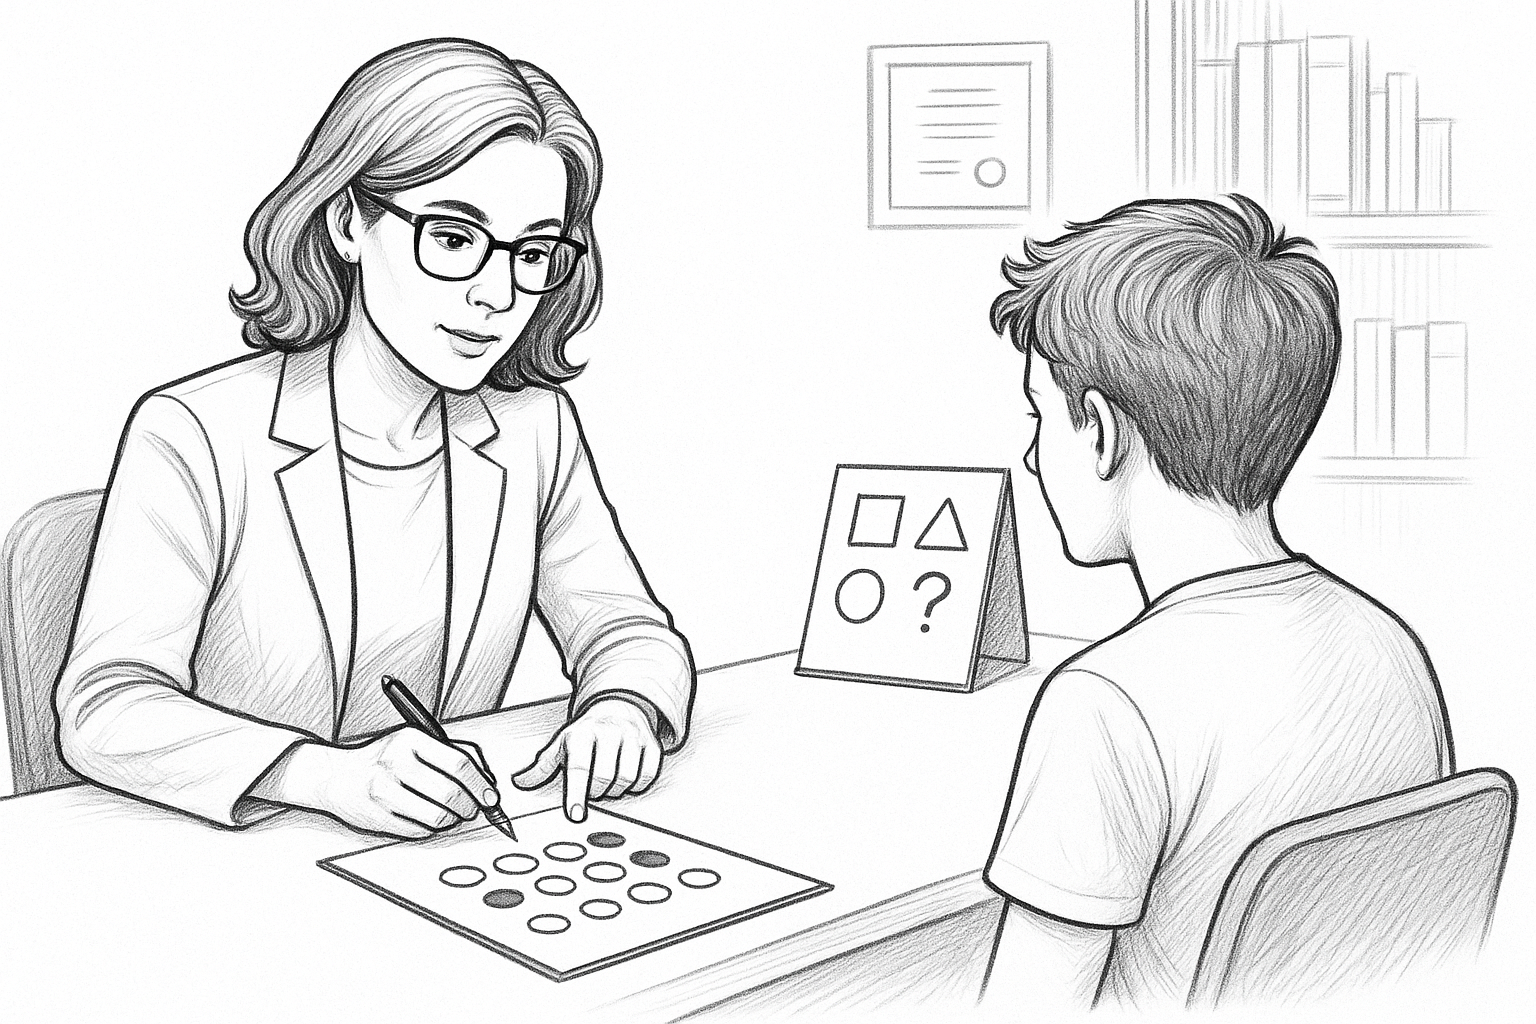
\includegraphics[width=0.6\linewidth,height=\textheight,keepaspectratio]{chapters/../Figures/Valutazione_Neuropsi_ChatGPT.png}

}

\caption{\label{fig-chatgpt-valutazione}Una valutazione neuropsicologica
secondo ChatGPT (vedi testo per il prompt esatto)}

\end{figure}%

In altre parole, la neuropsicologia clinica come disciplina
\emph{presuppone} che la misurazione degli oggetti di interesse
(funzionamento cognitivo, rischio di sviluppare una malattia, ecc.)
consenta di raggiungere conclusioni diagnostiche migliori, di fare
scelte terapeutiche più efficaci e, in generale, di svolgere una
migliore attività clinica (si veda il paragrafo \emph{``Epistemologia
della neuropsicologia clinica''} per ulteriori dettagli). La
misurazione, cioè l'utilizzo di punteggi, ci aiuta a quantificare delle
proprietà di interesse e poter fare delle scelte cliniche più precise
rispetto al solo utilizzo della osservazione clinica qualitativa e
basate su evidenze scientifiche. Il più delle volte questo implica che i
punteggi sono confrontati con delle soglie e se i valori sono al di là
di queste soglie, viene concluso che il risultato ha rilevanza clinica
(useremo più avanti termini più tecnici e definizioni più precise). La
persona con il punteggio al di là della soglia potrebbe avere un deficit
cognitivo, o forse un rischio di avere una patologia neurodegenerativa o
un disturbo del neurosviluppo.

Va da sé, che se questo è uno dei presupposti della neuropsicologia
clinica come disciplina, effettuare correttamente le misurazioni è un
primo aspetto fondamentale che determinerà la qualità della nostra
attività clinica.

\section{Misurazione e neuropsicologia
clinica}\label{misurazione_e_neuropsicologia_clinica}

La disciplina che si occupa della misurazione in psicologia (e in
neuropsicologia) è la \textbf{psicometria}, una delle discipline che,
insieme alla statistica, rappresentano le fondamenta di questo libro. La
psicometria si occupa proprio delle questioni della misurazione in
psicologia, una tipologia di misurazione molto particolare perché non
tratta di proprietà di oggetti fisici ma di \textbf{costrutti}, cioè
concetti psicologici non osservabili.

\begin{tcolorbox}[enhanced jigsaw, title=\textcolor{quarto-callout-note-color}{\faInfo}\hspace{0.5em}{Definizione}, coltitle=black, bottomtitle=1mm, colback=white, bottomrule=.15mm, rightrule=.15mm, breakable, toptitle=1mm, left=2mm, colbacktitle=quarto-callout-note-color!10!white, titlerule=0mm, colframe=quarto-callout-note-color-frame, leftrule=.75mm, opacitybacktitle=0.6, arc=.35mm, toprule=.15mm, opacityback=0]

\textbf{Costrutto}: Un concetto psicologico non direttamente osservabile
(es. memoria, attenzione, intelligenza). Per renderlo misurabile, è
associato ad uno o più \emph{indicatori} (o \emph{proxy} in inglese).
\vspace{1em}

\textbf{Indicatore} Un comportamento osservabile che, da solo o insieme
ad altri, si assume sia manifestazione di un costrutto a cui è
associato. In neuropsicologia clinica, sono tipici indicatori le
risposte ad un test.

\end{tcolorbox}

Il fatto che i costrutti siano proprietà non osservabili non è di per sé
un problema insormontabile ed è comune in vari ambiti diversi da quello
psicologico. Per esempio, si pensi, al campo magnetico prodotto da un
oggetto, o alla sua temperatura, entrambe proprietà non direttamente
osservabili ma misurabili attraverso indicatori fisici.

Consideriamo il classico termometro con colonnina di galinstan (un tempo
a mercurio). La \emph{temperatura} del nostro corpo non è direttamente
osservabile ma possiamo misurarla grazie a un indicatore fisico
osservabile: l'espansione di una colonna di un metallo liquido
(galinstan o mercurio) all'interno del termometro. Quando la temperatura
aumenta, il liquido si espande e la sua variazione in lunghezza viene
trasformata in un numero che rappresenta la proprietà fisica che ci
interessa, cioè la temperatura. Nessuno mette in dubbio la bontà di
questa misurazione perché diamo per scontata con precisione la relazione
fisica tra la temperatura e l'espansione del metallo.

La misurazione psicologica funziona in modo analogo, con indicatori
osservabili (es. le risposte a un test), associati a costrutti non
osservabili che intendiamo misurare. La psicometria, come disciplina, si
occupa proprio di come rendere questa relazione il più precisa e
giustificata possibile (questo esempio è ripreso e approfondito anche
nel paragrafo \hyperref[i-test]{\emph{``i test''}}).

Una caratteristica peculiare della misurazione psicologica è infatti che
la relazione tra ciò che è l'esito della misura (cioè il punteggio) e
ciò che si vuole misurare, cioè il costrutto, è molto indiretto. Nel suo
manuale ``Neuropsychological Assessment'', Muriel Lezak, una delle
persone più influenti nella neuropsicologia clinica riporta questo
passaggio (di Sivan \& Benton, 1999) molto esplicito a riguardo.

\emph{``Le abilità cognitive (e le disabilità) sono proprietà funzionali
dell'individuo che non vengono osservate direttamente, ma piuttosto
inferite dal comportamento. Ogni comportamento (compresa la performance
nei test neuropsicologici) è determinato da molteplici fattori:
l'insuccesso di un paziente in una prova di ragionamento astratto può
non dipendere da un deficit specifico nel pensiero concettuale, ma da un
disturbo dell'attenzione, da una difficoltà verbale o dall'incapacità di
discriminare gli stimoli della prova.''} (\cite{sivan1999cognitive})

In breve:

\emph{Non esiste una corrispondenza univoca tra un comportamento e uno
specifico aspetto del funzionamento cognitivo (normale o deficitario).
Quasi per definizione ogni comportamento è riconducibile a più funzioni
cognitive}.

È importante sottolineare che in neuropsicologia clinica non si
effettuano solo misurazioni di costrutti. In numerosi casi infatti i
punteggi hanno un diverso scopo, come stimare la probabilità di
sviluppare una patologia neurologica, la probabilità di sviluppare
sintomi comportamentali, o semplicemente predire quale potrebbe essere
il punteggio di un test particolarmente lungo a partire da un test più
breve. Distinguere tra questi casi è rilevante perché alcuni metodi
psicometrici e alcune considerazioni statistiche valgono solo per i test
che misurano costrutti oppure solo per i test che \emph{non} misurano
costrutti. Tutti questi aspetti saranno approfonditi nei paragrafi e
capitoli successivi

\subsection{La definizione di misurazione di S.S. Stevens (1946) e le
scale di
misura}\label{la-definizione-di-misurazione-di-s.s.-stevens-1946-e-le-scale-di-misura}

La più famosa definizione di misurazione è certamente quella di S.S.
Stevens, che in un articolo del 1946 ha fornito una definizione che ha
influenzato (nel bene e nel male) la storia della psicologia:

\begin{tcolorbox}[enhanced jigsaw, title=\textcolor{quarto-callout-note-color}{\faInfo}\hspace{0.5em}{Definizione}, coltitle=black, bottomtitle=1mm, colback=white, bottomrule=.15mm, rightrule=.15mm, breakable, toptitle=1mm, left=2mm, colbacktitle=quarto-callout-note-color!10!white, titlerule=0mm, colframe=quarto-callout-note-color-frame, leftrule=.75mm, opacitybacktitle=0.6, arc=.35mm, toprule=.15mm, opacityback=0]

\textbf{Misurazione secondo Stevens}

\emph{``\ldots possiamo dire che la misurazione, nel senso più ampio, è
definita come l'assegnazione di numeri a oggetti o eventi secondo
determinate regole.''} (\cite[p.~667]{stevens1946measurement})

\end{tcolorbox}

La proposta di Stevens va contestualizzata al clima del momento. Alla
fine degli anni quaranta si stava discutendo in ambito scientifico se
gli oggetti di interesse della psicologia potessero essere misurati e
se, quindi, la psicologia potesse essere considerata una scienza.
L'iniziale conclusione di una commissione internazionale di fisici e
psicologi che si era riunita per dare una risposta a questa domanda era
arrivata alla conclusione che, secondo una definizione rigorosa di
misurazione, la risposta era \emph{no}. Secondo Stevens però, il
problema era proprio nei presupposti della commissione e, più in
particolare, nella definizione troppo restrittiva di misurazione.
Propose dunque la definizione riportata sopra, e sottolineò che anche se
ogni regola porta a misurazione, un aspetto importante (ma separabile) è
l'utilizzo che si può fare dei numeri o classificazioni e questo dipende
dalla \textbf{Scala di misura}. A seconda delle proprietà misurate
potrebbe quindi essere diverso l'utilizzo che possiamo fare dei numeri.
La proposta di Stevens salvava la psicologia come scienza e anzi aiutava
a chiarire l'utilizzo dei numeri per la misurazione in diverse
circostanze.

Esistono quattro scale di misura: \emph{categoriale, ordinale, a
intervalli, a rapporti}. Queste scale possono essere organizzate
gerarchicamente (categoriale al livello più basso, a rapporti al livello
più alto), e le operazioni possibili ad un livello più basso sono
possibili a tutti i livelli superiori. Per esempio calcolare la mediana
è possibile a livello di scala ordinale, ma anche nella scala ad
intervalli e a rapporti in quanto più alte nella gerarchia. Da notare
che anche il solo rilevare se una persona è femmina o maschio è, secondo
la definizione di Stevens, un caso di misurazione, utilizzando una
\emph{scala categoriale}. In questo caso non hanno senso operazioni tipo
addizione o sottrazione o moltiplicazione (non ha senso dire che una
femmina è due volte un maschio o viceversa) e una delle poche operazioni
possibili è contare quanti casi abbiamo per ogni categoria (es.
confrontare il numero di femmine con il numero di maschi). Un riassunto
delle scale e delle operazioni possibili è riportato nella tabella 1.2.

\begingroup
{\scriptsize

\begin{longtable}[]{@{}
  >{\raggedright\arraybackslash}p{(\linewidth - 6\tabcolsep) * \real{0.0773}}
  >{\raggedright\arraybackslash}p{(\linewidth - 6\tabcolsep) * \real{0.4309}}
  >{\raggedright\arraybackslash}p{(\linewidth - 6\tabcolsep) * \real{0.1823}}
  >{\raggedright\arraybackslash}p{(\linewidth - 6\tabcolsep) * \real{0.3094}}@{}}
\caption{Tabella 1.2: Le quattro tipologie di scale di misura secondo
S.S. Stevens.}\tabularnewline
\toprule\noalign{}
\begin{minipage}[b]{\linewidth}\raggedright
Scala
\end{minipage} & \begin{minipage}[b]{\linewidth}\raggedright
Descrizione
\end{minipage} & \begin{minipage}[b]{\linewidth}\raggedright
Esempio
\end{minipage} & \begin{minipage}[b]{\linewidth}\raggedright
Operazioni possibili
\end{minipage} \\
\midrule\noalign{}
\endfirsthead
\toprule\noalign{}
\begin{minipage}[b]{\linewidth}\raggedright
Scala
\end{minipage} & \begin{minipage}[b]{\linewidth}\raggedright
Descrizione
\end{minipage} & \begin{minipage}[b]{\linewidth}\raggedright
Esempio
\end{minipage} & \begin{minipage}[b]{\linewidth}\raggedright
Operazioni possibili
\end{minipage} \\
\midrule\noalign{}
\endhead
\bottomrule\noalign{}
\endlastfoot
\textbf{Nominale} & Classificazione in categorie senza ordine implicito
& Sesso (M/F), Colori, Nazionalità & Conteggio, moda, verifica
uguaglianza/differenza \\
\textbf{Ordinale} & Classificazione con ordine, ma le distanze tra
categorie non hanno significato & Posizione in una classifica, Titolo di
studio & Ordinamento, mediane, percentili \\
\textbf{Intervallo} & Misura con ordine e intervalli uguali, ma senza
zero assoluto significativo & Temperatura in °C, IQ & Addizione,
Sottrazione,Media, Deviazione standard, z-score \\
\textbf{Rapporto} & Misura con ordine, intervalli uguali e lo zero ha un
significato & Età, Scolarità in anni, tempi di reazione & Tutte le
operazioni aritmetiche (×, ÷, +, −), z-score, rapporti \\
\end{longtable}

\textbf{Legenda}\\
- \emph{Scala}: tipo di misura secondo la classificazione di Stevens.\\
- \emph{Descrizione}: caratteristiche principali della scala.\\
- \emph{Esempio}: variabili reali che rientrano in quella scala.\\
- \emph{Operazioni possibili}: trasformazioni matematiche e statistiche
consentite dai dati.

}
\endgroup

L'idea di avere una definizione di misurazione molto generica,
accompagnata ad una distinzione di scale di misura è molto potente e
tuttora è molto influente nella misurazione in psicologia. Come
anticipato, però, ci sono anche altre definizioni. Nel prossimo
paragrafo sarà approfondita una di queste, che entrava in contrasto con
la proposta di Stevens.

\subsection{Definizione di Misurazione secondo Suppes e Zinnes
(1963)}\label{definizione-di-misurazione-secondo-suppes-e-zinnes-1963}

Un'altra possibile definizione di misurazione, molto celebre in
psicometria è quella di Suppes e Zinnes (\citeyear{suppes1963basic}). A
differenza di quella di Stevens è più rigorosa e formale, ma anche più
complessa e meno intuitiva e per essere capita necessita alcune
definizioni preliminari.

Definiamo \emph{Sistema Relazionale Empirico}, come l'insieme di entità
del mondo empirico che hanno una determinata proprietà che vogliamo
misurare (es. oggetti di diversa lunghezza) e il \emph{Sistema
Relazionale Numerico} un insieme di numeri (es. i numeri Reali) con i
quali vogliamo descrivere il sistema Relazionale Empirico.

\begin{figure}[H]

\centering{


\includegraphics[width=0.7\linewidth,height=\textheight,keepaspectratio]{chapters/../Figures/Latex-Fig-Misurazione-Fisica/Fig_measurement_1.png}

}

\caption{\label{fig-measurement-fisico}Sistema Relazionale Empirico e il
Sistema Relazionale Numerico: esempio della misurazione della lunghezza
di un tavolo.}

\end{figure}%

\begin{tcolorbox}[enhanced jigsaw, title=\textcolor{quarto-callout-note-color}{\faInfo}\hspace{0.5em}{Definizione}, coltitle=black, bottomtitle=1mm, colback=white, bottomrule=.15mm, rightrule=.15mm, breakable, toptitle=1mm, left=2mm, colbacktitle=quarto-callout-note-color!10!white, titlerule=0mm, colframe=quarto-callout-note-color-frame, leftrule=.75mm, opacitybacktitle=0.6, arc=.35mm, toprule=.15mm, opacityback=0]

\textbf{Misurazione secondo Suppes e Zinnes (1963)}

La misurazione consiste in un \textbf{omomorfismo} tra un \emph{Sistema
Relazionale Numerico} e un \emph{Sistema Relazionale Empirico}.

\end{tcolorbox}

Con \emph{omomorfismo} si intende una corrispondenza tra i due sistemi
che preserva le relazioni tra gli elementi. Ad esempio, se nel Sistema
Relazionale Empirico abbiamo una relazione di ordine (ad esempio,
l'oggetto A è più lungo dell'oggetto B), allora questa relazione deve
essere preservata nel Sistema Relazionale Numerico (il numero associato
all'oggetto A deve essere maggiore del numero associato all'oggetto B).

Nell'esempio della Figura~\ref{fig-measurement-fisico}, un tavolo ha un
lato lungo 120 cm. Possiamo usare questo numero (120) per numerosi
utilizzi. Supponiamo ad esempio di avere due tavoli quadrati, uno con il
lato di 120 cm e uno con il lato di 60 cm. Tramite questa misurazione
del loro lato, sappiamo che il tavolo con lato 120 cm è più lungo di
quello con lato 60 cm. Sappiamo che il tavolo con lato 120 cm ha il lato
di 60 cm più lungo di quello con lato 60 cm. Infine sappiamo che il
tavolo con lato 120 cm è lungo il doppio del tavolo con lato 60 cm
(nello stesso spazio del tavolo lungo 120 cm, possiamo mettere due
tavoli da 60 cm). Questi numeri ci permettono dunque di una serie di
operazioni utili per comprendere le proprietà dei tavoli, in questo caso
la loro lunghezza, e interagire con loro\footnote{Tornando per un attimo
  alla Definizione di misurazione di Stevens e alla Tabella 1.2, La
  lunghezza di un tavolo sarebbe misurata su una \emph{scala a rapporti}
  e sapere questo ci permette di sapere quali operazioni possiamo fare
  con i numeri associati alla misura.}. La stessa cosa accade quando
vogliamo fare una misurazione psicologica o neuropsicologica: lo scopo è
ottenere un numero che vogliamo utilizzare per alcuni scopi (si veda
Figura~\ref{fig-measurement-psicologico}).

\begin{figure}[H]

\centering{


\includegraphics[width=0.7\linewidth,height=\textheight,keepaspectratio]{chapters/../Figures/Latex-Fig-Misurazione-Psicologica/Fig_measurement_2.png}

}

\caption{\label{fig-measurement-psicologico}Sistema Relazionale Empirico
e Sistema Relazionale Numerico: esempio della misurazione di un
costrutto psicologico (memoria).}

\end{figure}%

In questo caso possiamo dire che il nostro Sistema Relazionale
Empirico\footnote{è importante notare che non tutti sarebbero d'accordo
  nel dire che l'insieme di costrutti psicologici (cioè concetti non
  osservabili) sono parte di un sistema relazionale empirico. La domanda
  è però proprio al confine dell'epistemologia: un concetto psicologico
  non osservabile è parte del mondo empirico (così come lo sono altri
  entità non osservabili) oppure no? Per i nostri scopi la diversa
  collocazione dei concetti psicologici (come entità del mondo empirico
  o no), è irrilevante. Qui assumo che i concetti psicologici siano di
  fatti parte dei sistemi relazionali empirici in un certo senso
  aggirando il problema, e utilizzando la definizione di sistema
  relazionale empirico come ogni sistema relazionale \emph{non}
  numerico.} è dato dall'insieme di tutti i possibili livelli di memoria
e il Sistema Relazionale Numerico come l'insieme di numeri che
utilizziamo per descrivere questi livelli memoria. Alcune operazioni con
questi numeri sono intuitivamente sensate, ad esempio possiamo dire che
alcune persone hanno più memoria di altre (possiamo quindi ordinare), ma
nel momento in cui cerchiamo di capire l'applicabilità di altre
operazioni diventa più difficile rispondere. Ad esempio, tramite un test
possiamo arrivare a dire che una persona ha il doppio di memoria di un
altra? Oppure che ha +20 unità di memoria più di un'altra? (qualsiasi
sia questa unità). La risposta non è ovvia, e non possiamo darla per
scontata solo perché abbiamo dei numeri. Suppes e Zinnes sostengono che
non si possa assumere automaticamente che determinate operazioni sui
numeri abbiano un senso. Occorre invece verificare che il sistema
numerico rappresenti adeguatamente la struttura delle relazioni
empiriche osservate; solo in questo caso le operazioni effettuate sui
numeri possono essere interpretate come operazioni dotate di senso sul
costrutto misurato\footnote{questo aspetto è affrontato più in dettaglio
  nella sezione \emph{Approfondimenti tecnici}}.

\section{Quale definizione di misurazione adottano i test
neuropsicologici?}\label{quale-definizione-di-misurazione-adottano-i-test-neuropsicologici}

Visto che esistono diversi modelli di misurazione, viene spontaneo
chiedersi quale di essi adottino i test neuropsicologici (specie quelli
disponibili in Italia) e quali conseguenze pratiche ne derivino.

La risposta non è semplice: per la maggior parte dei test, il modello di
misurazione sottostante non viene mai dichiarato esplicitamente.
Tuttavia, se facciamo un ragionamento al contrario e cerchiamo di
desumerlo a partire dall'utilizzo che si fanno dei punteggi, possiamo
dire che implicitamente si assuma la definizione di Stevens e che la
misura sia su scala ad intervalli.

\begin{tcolorbox}[enhanced jigsaw, title=\textcolor{quarto-callout-important-color}{\faExclamation}\hspace{0.5em}{Importante}, coltitle=black, bottomtitle=1mm, colback=white, bottomrule=.15mm, rightrule=.15mm, breakable, toptitle=1mm, left=2mm, colbacktitle=quarto-callout-important-color!10!white, titlerule=0mm, colframe=quarto-callout-important-color-frame, leftrule=.75mm, opacitybacktitle=0.6, arc=.35mm, toprule=.15mm, opacityback=0]

Nella maggior parte dei test neuropsicologici \emph{si assume}
implicitamente che la misura sia su scala a intervalli.

\end{tcolorbox}

Ricordiamo che assumere una scala ad intervalli significa che le
differenze tra punteggi hanno un significato costante lungo tutta la
scala. Un esempio classico è la temperatura in gradi Celsius: un aumento
di 2°C ha lo stesso significato indipendentemente dal valore di partenza
(che si passi da 36° a 38° o da 38° a 40°, in entrambi i casi la
variazione è identica).

Proviamo però ad applicare lo stesso ragionamento a qualche test
neuropsicologico, in maniera intuitiva. Prendiamo ad esempio il MoCA
(\cite{nasreddine2005montreal}), uno strumento di screening cognitivo
con punteggio da 0 a 30. Se fosse davvero misurato su una scala a
intervalli, un aumento di 2 punti dovrebbe avere lo stesso significato
sia partendo da 24 sia partendo da 28. Eppure un aumento da 28 a 30
porta a un punteggio perfetto, mentre uno da 24 a 26 indica due diversi
livelli di prestazione media/medio-alta\footnote{per complicare
  ulteriormente il quadro qualcuno che conosce il MoCA potrebbe anche
  dire che il significato di questi \(+2\), dipende molto da quale è
  l'item (o gli item) a cui è legato questo punteggio, questo esempio è
  trattato in un
  \hyperref[Approfondimento-item-arbitrari]{Approfondimento}).}. Per chi
conosce il test è quantomeno discutibile sostenere che le due variazioni
abbiano lo stesso significato.

Lo stesso vale per il Digit Span, test in cui si chiede di ricordare
sequenze di numeri di lunghezza crescente e il punteggio corrisponde
alla sequenza più lunga correttamente richiamata. Un aumento di 2 punti
da 3 a 5 segna il passaggio da una prestazione molto bassa a una
intermedia; un aumento da 8 a 10 porta invece da una prestazione già
eccellente a una quasi irraggiungibile (provate a ricordare una sequenza
di 10 cifre per capire). Anche qui le due variazioni potrebbero non
sembrare equivalenti.

Questi esempi, per quanto informali, mostrano come interpretare i
punteggi grezzi di un test come se fossero su scala a intervalli non si
possa dare per scontato. Eppure, la maggior parte dei test
neuropsicologici non riporta evidenze o non effettua verifiche che
mostrino l'effettiva adeguatezza dell'utilizzo di una scala ad
intervalli.

Chi ha già utilizzato test neuropsicologici in ambito clinico potrebbe
obiettare che il problema è di scarsa rilevanza pratica, almeno quando i
test vengono usati semplicemente per stabilire se un punteggio è al di
sopra o al di sotto di una soglia di deficit: in quel caso non si
effettuano addizioni o sottrazioni, ma ci si limita a confrontare il
punteggio con un valore di riferimento (questo argomento sarà trattato
in dettaglio nel \hyperref[Capitolo3]{Capitolo 3}). Tuttavia, vi sono
situazioni in cui operazioni che implicano una scala ad intervalli
entrano in gioco anche nella pratica quotidiana. Un esempio tipico sono
le \emph{correzioni} per età e scolarità, trattate nel capitolo 3 e
nell'approfondimento sulle regressioni: queste correzioni consistono
nell'aggiungere o sottrarre un valore al punteggio grezzo, operazioni
che hanno senso solo su una scala ad intervalli. Anche molti dei metodi
utilizzati per misurare cambiamenti nel tempo (vedi paragrafo ), spesso
assumono una scala ad intervalli, con implicazioni non banali
sull'interpretazione dei risultati. L'aspetto più delicato di questa
discussione è che il trattare i punteggi come se fossero su una scala ad
intervalli è una sorta di punto di partenza e un'assunzione implicita
non dimostrata, piuttosto che qualcosa verificata empiricamente (come
Suppes e Zinnes suggeriscono nel loro modello di misurazione). Anche se
quanto appena detto potrebbe sembrare una speculazione da psicometristi,
con poco impatto pratico, nel corso di questo libro cercherò di
dimostrare che non lo è, e che anzi, in certi casi è una semplificazione
che non possiamo dare per scontata.

È doveroso anticipare già adesso che non sempre i test psicologici
soffrono di queste problematiche. Alcuni infatti sono costruiti in modo
tale che il significato delle variazioni di punteggio sia formalmente
definito e preciso, grazie all'impiego di modelli alternativi di
misurazione, ad esempio quelli appartenenti all' \textbf{Item Response
Theory}. Purtroppo, per ragioni pratiche e storiche, strumenti con tali
caratteristiche sono ancora poco diffusi nella pratica neuropsicologica
italiana, e dobbiamo quindi accontentarci di test che assumono una scala
ad intervalli, con tutte le problematicità evidenziate (si veda il
paragrafo Introduzione all'Item Response Theory per un approfondimento).

Devo però anche anticipare che adotterò una posizione molto pragmatica
su questo aspetto. Anche quando alcune assunzioni di un test risultano
discutibili, ciò non significa che il test vada scartato: uno strumento
con limitazioni può essere comunque più utile di una valutazione clinica
puramente qualitativa.

Ricapitolando: la maggior parte dei test neuropsicologici adotta
implicitamente la concezione della misurazione proposta da Stevens e
tratta i punteggi come misure su scala a intervalli, senza però
esplicitare o verificare l'adeguatezza di tale assunzione. Gli esempi
forniti sul MoCA e del Digit Span mostrano come questa assunzione non si
possa però dare per scontata con leggerezza. Va tuttavia chiarito che il
neuropsicologo non deve porsi quotidianamente il problema della scala di
misurazione, a meno che non decida di effettuare operazioni sui punteggi
al di là di quelle previste dalla pratica clinica standard. Il messaggio
centrale è: \emph{ottenere dei numeri non ci autorizza a fare di essi
ciò che vogliamo}. Alcune operazioni, pur tecnicamente possibili,
possono essere delicate o problematiche, e sapere che derivano da
un'assunzione discutibile è fondamentale per un'interpretazione
consapevole dei punteggi.

Abbiamo parlato a lungo di misurazione, ma lasciamo adesso spazio a
quelli che sono gli strumenti di misurazione in neuropsicologia: i test.

\section{I test}\label{i-test}

Già dall'introduzione è stato detto che il protagonista assoluto del
libro è il test neuropsicologico. Ma cos'è un test? Come sempre, non
possiamo non procedere senza fornire una definizione precisa che ci
aiuti a definire cosa è un test (e cosa non lo è) e quali sono le
caratteristiche che lo contraddistinguono.

Esistono in letteratura numerose definizioni di test e, come spesso
accade in psicometria, non esiste un consenso unanime su quale sia la
più adeguata. Una delle più influenti in ambito psicologico è quella
proposta da Lee Cronbach nel suo manuale sul testing psicologico:

\begin{tcolorbox}[enhanced jigsaw, title=\textcolor{quarto-callout-note-color}{\faInfo}\hspace{0.5em}{Definizione}, coltitle=black, bottomtitle=1mm, colback=white, bottomrule=.15mm, rightrule=.15mm, breakable, toptitle=1mm, left=2mm, colbacktitle=quarto-callout-note-color!10!white, titlerule=0mm, colframe=quarto-callout-note-color-frame, leftrule=.75mm, opacitybacktitle=0.6, arc=.35mm, toprule=.15mm, opacityback=0]

\textbf{Test secondo Cronbach (1990)}

\emph{``Un test è una procedura sistematica per l'osservazione del
comportamento di una persona e per la sua descrizione con l'aiuto di una
scala numerica o tramite categorie prefissate.''}
(\cite{cronbach1990essentials}) (p.~32)

\end{tcolorbox}

Fermiamoci a riflettere un attimo sui vari aspetti catturati da questa
definizione:

\emph{``Un test è una procedura sistematica \ldots{}''}

Questa parte della definizione sottolinea che un test non è
semplicemente un insieme di materiali, ma è un processo ben definito e
una ``procedura'', cioè una sequenza di passaggi che devono essere
seguiti affinché si possa dire che è stato somministrato esattamente
quel test.

\emph{``\ldots{} per l'osservazione del comportamento \ldots{}''}

In questa seconda parte della definizione, viene sottolineato quanto già
detto riguardo la misurazione psicologica: i test psicologici si basano
sull'osservazione di comportamenti.

\emph{``\ldots{} e per la sua descrizione con l'aiuto di una scala
numerica o tramite categorie prefissate.''}

In quest'ultima parte della definizione, è catturata l'essenza
dell'esito di una misurazione: un punteggio o l'appartenenza ad una
categoria (es. ``sano'', ``Mild Cognitive Impairment'').

\begin{tcolorbox}[enhanced jigsaw, title=\textcolor{quarto-callout-important-color}{\faExclamation}\hspace{0.5em}{Nota}, coltitle=black, bottomtitle=1mm, colback=white, bottomrule=.15mm, rightrule=.15mm, breakable, toptitle=1mm, left=2mm, colbacktitle=quarto-callout-important-color!10!white, titlerule=0mm, colframe=quarto-callout-important-color-frame, leftrule=.75mm, opacitybacktitle=0.6, arc=.35mm, toprule=.15mm, opacityback=0]

Il fatto che un test sia una \textbf{procedura sistematica} implica che,
per somministrarlo correttamente, occorre attenersi scrupolosamente alla
procedura originale: quella indicata dagli autori, nel manuale del test
o nella pubblicazione scientifica di riferimento. Anche una deviazione
apparentemente piccola può avere un impatto rilevante sui risultati e
sulla loro interpretazione, producendo effetti a cascata difficili da
prevedere. Per esempio, modificare leggermente le istruzioni, anche con
il nobile intento di essere più chiari, può rendere il test più facile e
alterare il significato del confronto con i dati normativi (si veda il
paragrafo sui dati normativi).

\end{tcolorbox}

Questa definizione ha il vantaggio di essere ampia e inclusiva: si
applica tanto ai test cognitivi quanto ai questionari di personalità,
alle scale di autovalutazione e a molti altri strumenti di misura in
ambito psicologico. Tuttavia, presenta un limite importante per i nostri
scopi, che è facile identificare con un esempio. Provate a immaginare
uno strumento che valuti l'equilibrio di una persona durante il cammino
tramite una serie di prove fisiche. Per ogni prova superata si dà un
punteggio di 1, e il punteggio globale è dato dalla somma dei punteggi
delle varie prove. Questo strumento soddisferebbe formalmente la
definizione di Cronbach: è una procedura sistematica, per osservare il
comportamento e lo descriverebbe con una scala numerica (il punteggio
totale). Tuttavia, questo strumento non sarebbe un test ``psicologico''.

La definizione di Cronbach è utile quindi perché permette di
sottolineare, tramite una mancanza, un punto fondamentale che
contraddistingue i test psicologici: a differenza di altri tipi di test,
i test psicologici non hanno quasi mai interesse solo nel comportamento
osservato (le risposte del paziente agli item del test) ma nel
\textbf{costrutto} psicologico che si vuole misurare (vedi
\hyperref[cosa-misuriamo-in-neuropsicologia-clinica]{paragrafo
precedente}). Il punteggio è dunque una rappresentazione
\emph{indiretta} di qualcosa di non direttamente osservabile (memoria,
attenzione, funzioni esecutive, ecc.), tramite un comportamento
osservabile. Questa relazione è rappresentata nella
Figura~\ref{fig-costrutto-punteggio}.

\begin{figure}[H]

\centering{

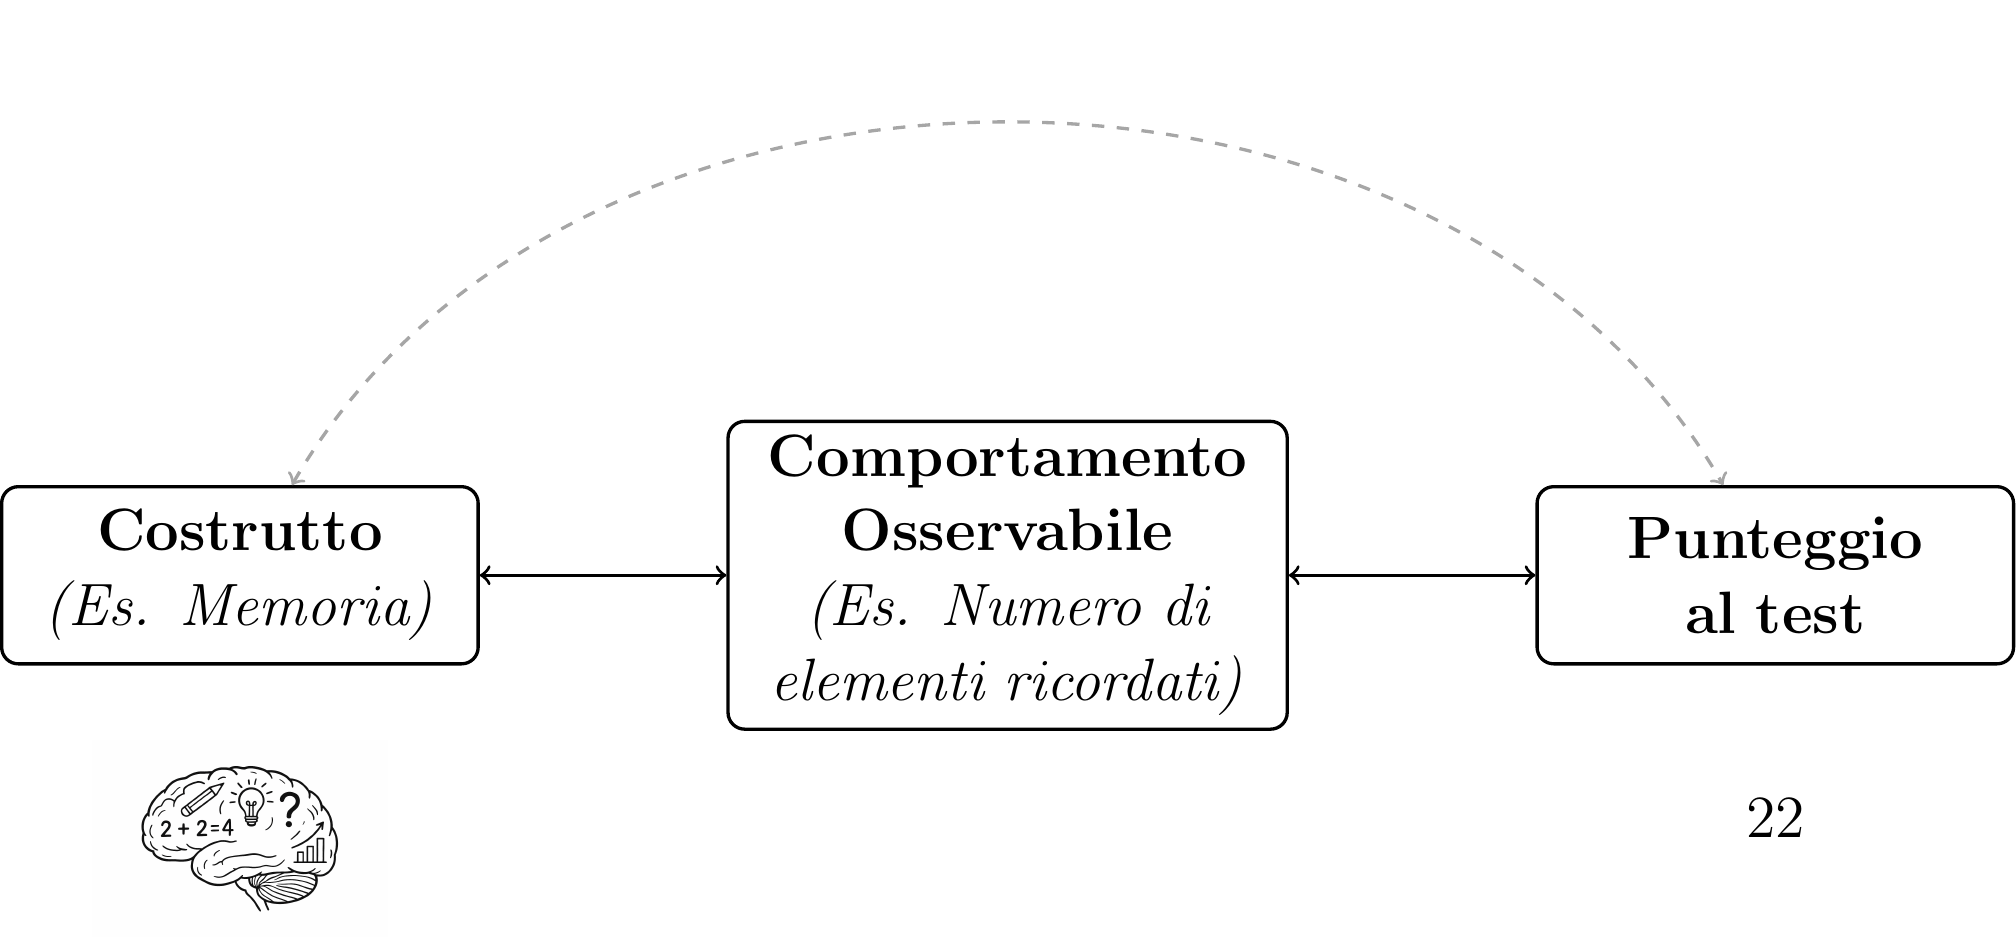
\includegraphics[width=0.8\linewidth,height=\textheight,keepaspectratio]{chapters/../Figures/Latex-Fig-Costrutto-Comportamento-Punteggio/Fig_measurement_3.png}

}

\caption{\label{fig-costrutto-punteggio}Relazione tra costrutto,
comportamento e punteggio al test. Il costrutto non osservabile (es.
Memoria, Ansia) è legato a comportamenti osservabili (es. risposte al
test), i quali determinano il punteggio. La freccia tratteggiata
bidirezionale indica la relazione indiretta tra costrutto e punteggio.}

\end{figure}%

Da notare che quanto appena detto è, in sostanza, quello che abbiamo già
trattato nel paragrafo
\hyperref[misurazione_e_neuropsicologia_clinica]{\emph{``misurazione e
neuropsicologia clinica''}}. Riprendiamo l'esempio della misurazione con
un termometro e approfondiamolo. La situazione di una misurazione
indiretta in psicologia potrebbe sembrare non troppo diversa da quella
dell'esempio del termometro: del resto anche la temperatura non è
direttamente osservabile, ma è legata a un indicatore osservabile
(l'espansione del galinstan o mercurio) che ci permettono di ottenere un
numero (i gradi) che rappresenta indirettamente ciò che vogliamo
misurare. Nonostante questa apparente somiglianza, la misurazione in
neuropsicologia, e in psicologia in generale, è molto più complessa.
Senza scendere troppo nei dettagli la ragione è che la relazione tra
costrutto psicologico e indicatore è molto più complessa di quello che
accade con gli indicatori osservabili di misurazioni fisiche. Più nello
specifico non esiste una relazione \emph{causale} univoca tra proprietà
non osservabile e comportamento osservabile: avere una certa memoria non
determina in maniera causale che si ottenga un certo comportamento
(piuttosto probabilistica, vedi paragrafo ``Altri modelli di
misurazione''). A complicare le cose, molte variabili non direttamente
di interesse possono alterare in maniera importante la relazione tra
costrutto e comportamento osservabile (cioè l'indicatore). Sempre in
relazione al punteggio al test di memoria si consideri per esempio la
motivazione, l'umore, la fatica, la stanchezza, l'ansia, la confusione,
la distrazione, la presenza di dolore o di sintomi fisici, e così via.
Tutte queste variabili possono influenzare il comportamento osservato
(le risposte al test) e di conseguenza il punteggio ottenuto,
indipendentemente dal costrutto di interesse (la memoria).

\begin{figure}[H]

\centering{

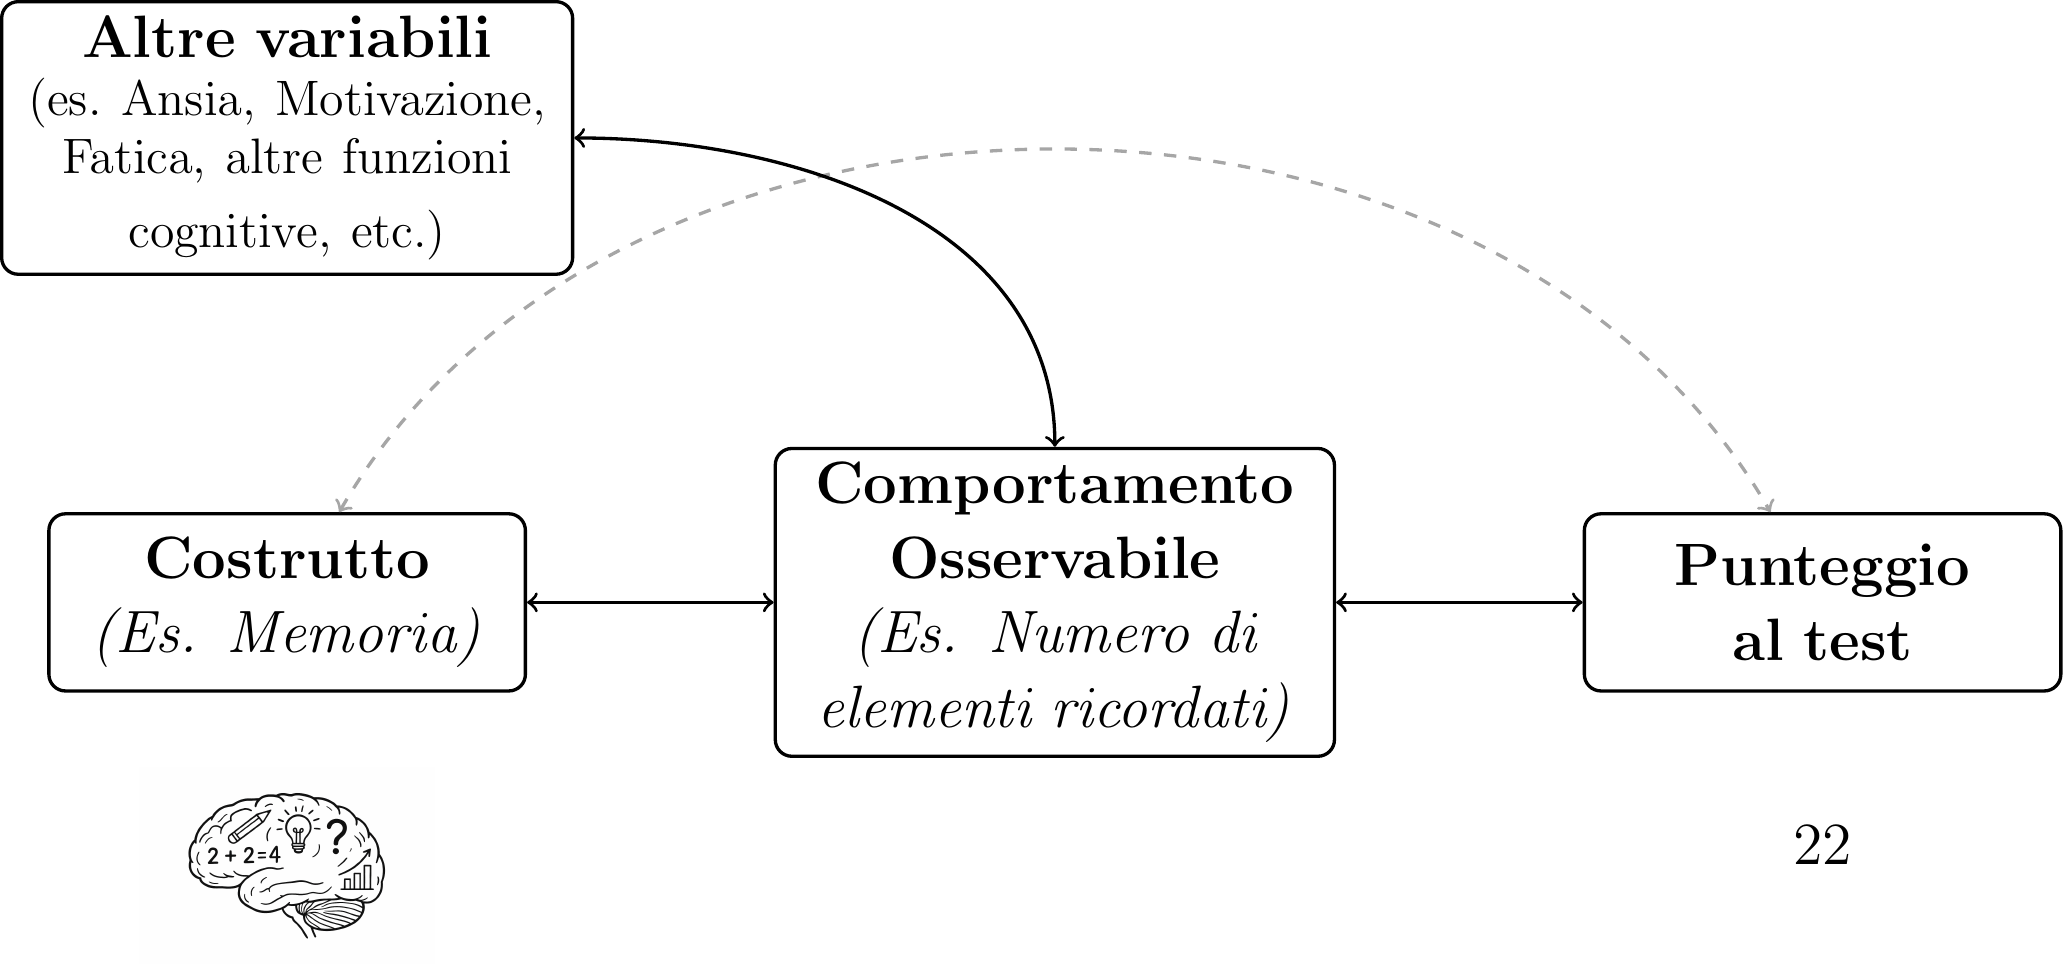
\includegraphics[width=0.8\linewidth,height=\textheight,keepaspectratio]{chapters/../Figures/Latex-Fig-AltreVariabili/Fig_measurement_4.png}

}

\caption{\label{fig-altre-variabili}Relazione tra costrutto,
comportamento e punteggio al test. Il costrutto non osservabile (es.
Memoria, Ansia) produce comportamenti osservabili (es. risposte al
test), i quali determinano il punteggio. La freccia tratteggiata
bidirezionale indica la relazione indiretta tra costrutto e punteggio.
Le altre variabili (Motivazione, Umore, Fatica, etc.) influenzano il
comportamento osservato indipendentemente dal costrutto di interesse.}

\end{figure}%

\pagebreak

\subsection{Tipologie di test}\label{tipologie-di-test}

Esistono diverse tipologie di test così come diversi modi di poterli
classificare. Di seguito vengono descritti i principali tipi di test
utilizzati in neuropsicologia clinica. Fornire una classificazione è
utile perché diversi tipi di test hanno diverse peculiarità di tipo
psicometrico. Nel corso del libro specificheremo quando alcune
considerazioni si applicano solo, o prevalentemente, ad un tipo di test.

\subsubsection{Test di prestazione
massima}\label{test-di-prestazione-massima}

I \textbf{test di prestazione massima} (\emph{maximal performance
tests}) sono strumenti in cui si chiede al paziente di impegnarsi al
massimo delle proprie capacità per ottenere il miglior risultato
possibile. L'obiettivo è valutare \emph{cosa una persona è in grado di
fare} quando le condizioni sono ottimali e lo sforzo è massimo. La
maggior parte dei test neuropsicologici per la valutazione delle
funzioni cognitive (test di memoria, attenzione, funzioni esecutive,
linguaggio, abilità visuospaziali) rientra in questa categoria. Il
punteggio ottenuto è interpretato come una stima della capacità massima
del paziente in quel dominio cognitivo.

\subsubsection{Test di comportamento
tipico}\label{test-di-comportamento-tipico}

I \textbf{test di comportamento tipico} (\emph{typical behaviour tests})
sono invece strumenti progettati per valutare come una persona si
comporta o risponde \emph{tipicamente}, ovvero nel suo quotidiano, non
necessariamente con un sforzo massimo. In questi strumenti non esiste
una risposta ``giusta'' da dare. Rientrano in questa categoria due
grandi famiglie di strumenti:

\begin{itemize}
\tightlist
\item
  \textbf{Autosomministrati} (compilati dal paziente stesso):
  questionari di personalità, scale di autovalutazione per sintomi
  psicologici come ansia e depressione (es. Beck Depression Inventory
  (\cite{beck1961inventory}), Hamilton Anxiety Scale
  (\cite{hamilton1959assessment})), scale per la qualità della vita. Il
  paziente descrive come si sente o come si comporta generalmente.
\item
  \textbf{Eterosomministrati} (compilati dal clinico o da un caregiver):
  scale per la valutazione del funzionamento nelle attività quotidiane,
  come le ADL, \emph{Activities of Daily Living};
  (\cite{katz1963studies}) e le IADL, \emph{Instrumental Activities of
  Daily Living} (\cite{lawton1969assessment}). In questo caso è il
  clinico o un familiare a rispondere sulla base dell'osservazione
  diretta del paziente, non il paziente stesso.
\end{itemize}

La distinzione tra questi due tipi di test è rilevante per la
somministrazione, per l'interpretazione dei punteggi e per il tipo di
costrutto che si intende misurare.

\subsubsection{Altri strumenti utili per la valutazione
neuropsicologica}\label{altri-strumenti-utili-per-la-valutazione-neuropsicologica}

Nella pratica clinica, accanto ai test di prestazione massima e ai
questionari di comportamento tipico, esiste una terza categoria di
strumenti che fanno parte della valutazione neuropsicologica standard
pur non rientrando in senso stretto nella classificazione fin qui
descritta: si tratta di \textbf{questionari e scale somministrate come
parte integrante della valutazione clinica}, non per misurare una
funzione cognitiva o altri costrutti psicologici legati a comportamenti
abituali, ma per raccogliere informazioni contestuali utili per
l'interpretazione dei risultati.

L'esempio più rilevante in ambito neuropsicologico e che negli ultimi
anni ha avuto sempre più utilizzo è la stima della \textbf{riserva
cognitiva}. La riserva cognitiva, cioè la capacità del cervello di
compensare per i danni di una la patologia degenerativa o acuta senza
manifestare sintomi espliciti, è considerata una variabile moderatrice
importante nell'interpretazione delle prestazioni cognitive, soprattutto
nelle valutazioni legate a patologie neurodegenerative. Per stimarla si
utilizzano strumenti come il \textbf{CRIq} (\emph{Cognitive Reserve
Index questionnaire}; \cite{nucci2012cognitive}), un questionario in cui
si raccolgono informazioni su anni di istruzione, attività lavorativa e
attività del tempo libero nel corso della vita. Il CRIq non è un test di
prestazione massima: non si chiede al paziente di fare del proprio
meglio su un compito, ma di riportare informazioni anamnestiche
strutturate.

Questi strumenti condividono con i test psicologici il fatto di produrre
un punteggio numerico, e rientrano quindi nella definizione di test di
Cronbach.

\subsection{Questo è un buon test?}\label{questo-uxe8-un-buon-test}

La definizione di Cronbach, pur essendo ampia e inclusiva, lascia aperta
una domanda importante: \emph{qualunque} strumento che assegni numeri a
comportamenti osservati può essere considerato un buon test?
Consideriamo il seguente test ipotetico per la memoria:

\begin{quote}
Al paziente viene letta ad alta voce la seguente lista di 7 parole:
\emph{casa, mela, treno, fiume, cane, libro, sole}. Dopo 30 secondi, gli
viene chiesto di ricordare quante più possibili. Il punteggio finale è
il numero di parole ricordate (da 0 a 7).
\end{quote}

Questo strumento soddisfa formalmente la definizione di Cronbach: è una
procedura sistematica, osserva il comportamento (le parole ricordate) e
lo descrive con una scala numerica. Soddisfa anche la definizione di
Stevens: assegna numeri a eventi secondo regole precise.

\begin{domanda}

Ma questo è davvero un buon test per la memoria?

\end{domanda}

È verosimile che la vostra risposta ``di pancia'', sia stata \emph{no},
anche se non avete una spiegazione tecnica. Potreste dire per esempio
che è troppo semplice, che 7 parole sono poche\footnote{Il numero di
  item da solo non è un indicatore della qualità di un test. Esistono
  test pubblicati e validati anche con pochissimi item: per esempio,
  esiste una versione a 3 item della \emph{UCLA Loneliness Scale} per la
  misurazione (\cite{gosling2024measuring}).}, che 30 secondi sono
pochi, che le parole sono troppo facili, etc. Tutte queste
considerazioni sono ragionevoli e probabilmente condivisibili, ma non
sono basate su aspetti tecnici o su effettive verifiche sulla qualità
del test. Sono semplicemente basate sul buon senso e sull'esperienza
clinica.

Nel corso di questo libro daremo delle risposte più rigorose a questa
domanda. Quello che per ora è importante sottolineare che, anche se
questo strumento soddisfa formalmente le definizioni di test e di
misurazione, non è detto che sia un buon test: dobbiamo avere altre
evidenze per poter dire che questo strumento misura la memoria in modo
accurato e preciso.

Esistono diversi framework teorici che hanno cercato di definire questi
aspetti fondamentali che definiscono come identificare se un test sta
funzionando come dovrebbe e, più in generale, come si dovrebbe costruire
un test. Come è possibile immaginare, tutto ciò è spesso strettamente
intrecciato a veri e propri modelli di misurazione psicologica. Nel
prossimo paragrafo tratteremo il framework più diffuso e utilizzato in
neuropsicologia clinica, noto come la Teoria Classica dei Test.

\section{Teoria Classica dei Test (CTT)}\label{teoria-classica-dei-test}

La Teoria Classica dei Test o \emph{Classical Test Theory (CTT)} è il
framework psicometrico su cui si basa la grande maggioranza dei test
neuropsicologici attualmente disponibili. Come già visto per altri
aspetti psicometrici, spesso non vi è una dichiarazione esplicita di
seguire la CTT, ma questo può essere desunto dall'utilizzo di alcune
analisi (ad esempio, calcolare la consistenza interna o l'affidabilità
test-retest), che ne sono una diretta espressione. Comprendere i
presupposti della CTT è quindi fondamentale non solo per chi costruisce
test, ma anche per chi li usa nella pratica clinica quotidiana.

\subsection{Il principio cardine: X = T +
E}\label{il-principio-cardine-x-t-e}

Il principio fondamentale della CTT è espresso in una formula
apparentemente semplice:

\begin{tcolorbox}[enhanced jigsaw, title=\textcolor{quarto-callout-note-color}{\faInfo}\hspace{0.5em}{Definizione}, coltitle=black, bottomtitle=1mm, colback=white, bottomrule=.15mm, rightrule=.15mm, breakable, toptitle=1mm, left=2mm, colbacktitle=quarto-callout-note-color!10!white, titlerule=0mm, colframe=quarto-callout-note-color-frame, leftrule=.75mm, opacitybacktitle=0.6, arc=.35mm, toprule=.15mm, opacityback=0]

\(X = T + E\)

\(X\): punteggio osservato (\emph{observed score})\\
\(T\): punteggio vero (\emph{true score})\\
\(E\): errore di misura (\emph{error})\\

\end{tcolorbox}

Nell'equazione base della CTT, \(X\) rappresenta il \textbf{punteggio
osservato}, ovvero quello che si ottiene concretamente somministrando il
test a una persona in una specifica occasione. \(T\) è il
\textbf{punteggio vero} (\emph{true score}), cioè la quantità del
costrutto che la persona davvero possiede, la sua vera capacità di
memoria, attenzione o qualsiasi altro attributo il test intenda
misurare. Infine, \(E\) è l'\textbf{errore di misura} (\emph{error}), la
componente casuale che in ogni singola somministrazione porta il
punteggio osservato a discostarsi, in più o in meno, dal punteggio vero.

L'idea centrale della CTT è che ogni volta che somministriamo un test
otteniamo una stima imperfetta dell'abilità reale della persona: il
punteggio osservato \(X\) è la somma di quanto la persona sa o può fare
davvero (\(T\)) e di una quota di rumore casuale (\(E\)) che dipende da
molte circostanze, anche contingenti (ad esempio la stanchezza del
giorno, il livello di ansia durante la valutazione, una distrazione
durante le istruzioni, un item che per qualche motivo è risultato più
facile o difficile del solito). \emph{L'errore, può essere positivo o
negativo e varia simmetricamente intorno allo zero.} Un altro modo di
pensare \(T\) è quello del punteggio che otterremmo se non avessimo
alcun errore di misura.

Un'assunzione cruciale è che \(T\) ed \(E\) siano \emph{indipendenti tra
loro}: l'errore non dipende sistematicamente dal punteggio vero della
persona. In altre parole, avere un punteggio basso o alto non rende
l'errore sistematicamente più grande o più piccolo, è sempre una
componente casuale che oscilla intorno allo zero.

Per fare un esempio concreto: supponiamo che il punteggio vero di una
persona a un test di memoria, in cui il punteggio va da 0 a 30, sia
\(T = 10\). Se il giorno della somministrazione la persona è stanca o
ansiosa, potrebbe ottenere \(X = 7\), con un errore \(E = -3\) che ha
abbassato il punteggio. Se invece è riposata e particolarmente motivata,
potrebbe ottenere \(X = 12\), con \(E = +2\) che lo ha leggermente
sovrastimato. In entrambi i casi, il punteggio vero rimane \(T = 10\).
Da notare che il possibile errore non sarebbe diverso se il punteggio
vero fosse più basso (es. \(T = 5\)) o più alto (es. \(T = 25\)). Il
punteggio vero \(T\), che stimiamo a partire dal punteggio osservato
\(X\) è la rappresentazione dell'abilità reale, quella che rimarrebbe
stabile se potessimo somministrare lo stesso test infinite volte nelle
stesse condizioni ideali.

L'idea delle ``misurazioni infinite'' non è solo un espediente retorico:
nella CTT il punteggio vero \(T\) è definito formalmente proprio come il
valore atteso (la media) di \(X\) su infinite ripetizioni della misura.
Se l'errore \(E\) è davvero casuale e con media zero, come la CTT
assume, allora i contributi positivi e negativi dell'errore si
cancellerebbero a vicenda su infinite somministrazioni, e la media di
tutti i punteggi osservati convergerebbe esattamente a \(T\). In una
singola somministrazione non sappiamo se l'errore ci ha penalizzato o
favorito; ma l'idea che \(T\) ``esista'' come limite di questo processo
ci dà un fondamento teorico per trattare il punteggio osservato come una
stima, per quanto imperfetta, dell'abilità reale.

La Figura~\ref{fig-CTT-true-obs} illustra questa dinamica con una
simulazione: trenta somministrazioni ripetute dello stesso test alla
stessa persona (punteggio vero \(T = 10\)), con i punteggi osservati che
fluttuano attorno alla linea del punteggio vero per effetto dell'errore
casuale. Nessuna singola misurazione coincide esattamente con \(T\), ma
tutte sono intorno ad esso: è proprio questo che rende \(T\) una sorta
di ``centro di gravità'' della distribuzione dei punteggi osservati.

\begin{figure}[H]

\centering{

\pandocbounded{\includegraphics[keepaspectratio]{chapters/Misurazione_files/figure-pdf/fig-CTT-true-obs-1.pdf}}

}

\caption{\label{fig-CTT-true-obs}Trenta somministrazioni simulate dello
stesso test alla stessa persona con punteggio vero \(T = 10\) (linea
continua). I cerchi rappresentano i punteggi osservati, che fluttuano
attorno a \(T\) per effetto dell'errore casuale \(E\).}

\end{figure}%

È importante sottolineare che nella pratica clinica, ciò che vedremo
sarà sempre e solo \emph{un punteggio osservato} e cioè \(X\), molto
spesso una singola realizzazione di uno dei possibili punteggi osservati
possibili (in riferimento alla Figura~\ref{fig-CTT-true-obs}, quello che
vedremo è uno solo dei possibili cerchietti). Tale punteggio sarà dunque
sempre e solo una stima del punteggio vero \(T\), e non potremo mai
sapere con certezza se quell'osservazione è stata influenzata da un
errore positivo o negativo, né di quanto.

Questa consapevolezza porta a identificare due obiettivi prioritari nel
processo di costruzione di un test: il primo è ridurre al minimo
l'errore \(E\), affinché il punteggio osservato sia il più possibile
vicino al punteggio vero; il secondo è riuscire a stimare l'entità di
quell'errore, in modo da sapere con quale margine di incertezza si sta
lavorando quando si interpreta un punteggio. Va da sé, che in
neuropsicologia clinica, sarebbe prioritario avere test con il più
piccolo errore di misura possibile, in modo da ottenere stime più
precise dell'abilità reale dei pazienti e che siano il meno possibile
influenzati da fattori contingenti. Questo ci assicurerebbe di avere una
stima più accurata del funzionamento cognitivo dei pazienti, migliorando
la nostra capacità di diagnosticare deficit, monitorare cambiamenti nel
tempo e valutare l'efficacia di interventi riabilitativi.

\subsection{Limiti della CTT}\label{limiti-della-ctt}

La CTT, pur essendo il framework dominante e pur avendo dimostrato
grande utilità pratica, presenta alcuni limiti intrinseci che è
importante conoscere, non per scartare il modello, ma per sapere dove le
sue assunzioni devono essere accettate con una certa cautela o
quantomeno con consapevolezza.

Il primo limite riguarda il fatto che nella CTT le abilità del soggetto
e la difficoltà degli item non sono modellate separatamente. Il
punteggio di una persona dipende sia dalla sua abilità sia dalla
difficoltà specifica degli item inclusi in quella versione del test: un
test composto da item particolarmente difficili abbassa i punteggi di
tutti i soggetti, indipendentemente dalla loro abilità reale.

Il secondo limite riguarda l'assunzione di indipendenza tra \(T\) ed
\(E\). Questa assunzione, pur ragionevole nella parte centrale della
scala, è sistematicamente violata ai valori estremi. Se il punteggio
vero di una persona è vicino al massimo del test, l'errore non può
distribuirsi liberamente in entrambe le direzioni: la persona non può
ottenere un punteggio osservato superiore al massimo, quindi l'errore
può solo abbassare il punteggio, mai alzarlo oltre il limite. Lo stesso
accade al limite inferiore: il punteggio osservato non può scendere
sotto lo zero, per cui l'errore diventa asimmetrico e smette di essere
indipendente dal punteggio vero. Ai valori estremi, in altre parole,
l'errore stesso dipende da dove si trova la persona nella scala, il che
viola direttamente l'assunzione fondamentale del modello.

Torniamo all'ipotetico test di memoria con valori possibili da 0 a 30.
Se una persona avesse un punteggio vero \(T=30\), l'errore \(E\) non
potrebbe mai essere positivo, perché il punteggio osservato \(X\) non
può superare il massimo di 30. Se invece \(T=0\), l'errore non potrebbe
mai essere negativo, perché \(X\) non può scendere sotto zero. In
entrambi i casi, l'errore è limitato in una sola direzione, e quindi
dipende dal valore di \(T\), violando l'assunzione di indipendenza.

Questi limiti non rendono la CTT inutilizzabile, e i test
neuropsicologici che ne derivano rimangono strumenti clinicamente
preziosi nella pratica quotidiana, ma spiegano perché nel corso degli
anni si siano sviluppati modelli di misurazione alternativi.

\subsection{Costrutti misurati dai test
neuropsicologici}\label{costrutti-misurati-dai-test-neuropsicologici}

\begin{itemize}
\tightlist
\item
  intro su quali sono i costrutti?
\item
  test eteroegenei e non esiste un chiaro riferimento: ci sono talvolta
  domini, ma non esiste (se non in libri come Lezak), un elenco
  comprensivo di domini.
\item
  altri costrutti sono più vaghi e utilizzati in clinica. Es. FAB.
\item
  eterogeneità legata ad epistemologia (rimanda).
\end{itemize}

\subsection{\texorpdfstring{Riassunto sulla CTT
}{Riassunto sulla CTT }}\label{riassunto-sulla-ctt}

Abbiamo descritto il principio cardine della CTT e alcune delle sue
assunzioni fondamentali. Come anticipato, la maggior parte dei test
neuropsicologici adotta implicitamente questo framework e questo lo si
desume dalle analisi e dalle metodologie impiegate nel loro sviluppo,
più che da una dichiarazione esplicita.

Queste rispondono alla domanda posta in precedenza: come stabilire se un
test è un buon test? Secondo la CTT, sono necessarie informazioni sulla
\textbf{validità} del test, intesa come giustificazione del legame tra
punteggio e costrutto, e sulla sua \textbf{affidabilità}, ovvero la
precisione e la consistenza della misura. Questi due concetti
costituiscono il nucleo della psicometria nell'ambito della CTT e
saranno trattati in dettaglio nel
\hyperref[validita-e-affidabilita]{capitolo successivo}, dedicato
interamente a Validità e Affidabilità.

\begin{tcolorbox}[enhanced jigsaw, title=\textcolor{quarto-callout-tip-color}{\faLightbulb}\hspace{0.5em}{Nota}, coltitle=black, bottomtitle=1mm, colback=white, bottomrule=.15mm, rightrule=.15mm, breakable, toptitle=1mm, left=2mm, colbacktitle=quarto-callout-tip-color!10!white, titlerule=0mm, colframe=quarto-callout-tip-color-frame, leftrule=.75mm, opacitybacktitle=0.6, arc=.35mm, toprule=.15mm, opacityback=0]

Nei manuali o articoli dei test neuropsicologici spesso non è
esplicitamente scritto che sono sviluppati secondo la Classical Test
Theory. Questo è desumibile però dall'utilizzo di certe caratteristiche,
come l'utilizzo di Validità e Affidabilità, secondo specifiche
declinazioni tipiche di questo framework.

\end{tcolorbox}

\section{Oltre la Teoria Classica dei
Test}\label{oltre-la-teoria-classica-dei-test}

\section{Capitolo 1: Riassunto}\label{capitolo-1-riassunto}

Il capitolo ha introdotto la misurazione come l'assegnazione di numeri a
entità di interesse (tipicamente costrutti cognitivi) e ha argomentato
perché misurare sia centrale per un approccio scientifico alla
neuropsicologia clinica.

Abbiamo poi distinto tra \emph{costrutti} (proprietà psicologiche non
osservabili) e \emph{indicatori} (comportamenti osservabili, come le
risposte a un test), e confrontato due definizioni classiche di
misurazione: quella permissiva di Stevens (1946), basata
sull'assegnazione di numeri secondo regole e sulle quattro scale di
misura, e quella più rigorosa di Suppes e Zinnes (1963), che richiede un
omomorfismo verificato empiricamente tra sistema relazionale empirico e
numerico.

Applicando queste definizioni ai test neuropsicologici, abbiamo mostrato
che la maggior parte di essi assume implicitamente (e senza verifica)
una \emph{scala a intervalli}, un'assunzione discutibile ma diffusa.

Abbiamo poi definito cosa sia un \emph{test}, a partire dalla
definizione di Cronbach (1990), sottolineando che i test psicologici si
distinguono per l'interesse (quasi sempre) verso un costrutto
sottostante e non solo verso il comportamento osservato. Abbiamo quindi
esaminato alcune possibili classificazioni di test.

Il nucleo psicometrico del capitolo è la Teoria Classica dei Test (CTT),
il framework su cui si basa implicitamente la maggior parte dei test
neuropsicologici, sintetizzato dall'equazione \(X = T + E\) (punteggio
osservato = punteggio vero + errore casuale). Abbiamo discusso i suoi
limiti principali: l'assenza di una modellazione separata di abilità e
difficoltà degli item, e la violazione dell'indipendenza tra \(T\) ed
\(E\) ai valori estremi della scala.

\bookmarksetup{startatroot}

\chapter{Validità e Affidabilità}\label{validita-e-affidabilita}

\begin{domanda}

Possiamo considerare gli strumenti di misurazione tutti precisi allo
stesso modo?

\end{domanda}

La risposta a questa domanda retorica è, chiaramente, no. Sappiamo bene
che esistono strumenti più o meno precisi, e nella vita quotidiana ci
regoliamo di conseguenza. Un geometra che deve rilevare un muro non si
affida a un metro pieghevole, ma a un rilevatore laser. Per misurare con
esattezza la temperatura di un bambino è preferito comunque il
termometro ascellare, scomodo ma apparantemente più preciso, al
termometro auricolare, che fornisce una lettura più rapida ma
considerata meno stabile. Gli esempi si potrebbero moltiplicare, ma il
principio resta lo stesso: quando una misurazione è rilevante, scegliamo
gli strumenti che riteniamo più adeguati.

\begin{figure}[H]

{\centering 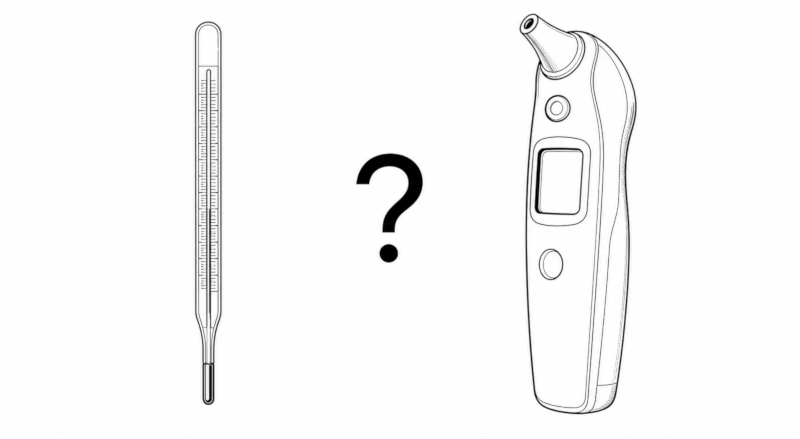
\includegraphics[width=0.8\linewidth,height=\textheight,keepaspectratio]{chapters/../Figures/termometri.png}

}

\caption{Strumenti con diversa precisione: questi due termometri sono
ugualmente precisi? La risposta che probabilmente darebbe un pediatra è
probabilmente no, favorendo quello ascellare perché in grado di fornire
misure più stabili, anche se più scomodo rispetto a quello auricolare.}

\end{figure}%

Su questo principio si fonda il presente capitolo. Anche i test
neuropsicologici sono strumenti di misurazione, e come tali impongono
attenzione alla loro precisione. Nell'ambito degli strumenti costruiti
secondo la teoria classica dei test, la bontà di uno strumento è
catturata principalmente da due proprietà: validità e affidabilità.

Entrambe sono direttamente collegate alla formula cardine \(X = T + E\),
(vedi il paragrafo \hyperref[teoria-classica-dei-test]{Teoria Classica
dei Test} nel capitolo precedente). In sintesi, la validità risponde
alla domanda \emph{``cosa stiamo misurando?''}, cioè se il punteggio
vero \(T\) rifletta effettivamente il costrutto che il test intende
misurare, mentre l'affidabilità risponde a \emph{``quanto precisamente
siamo misurando?''}, cioè quanto è piccola la componente d'errore \(E\)
rispetto al punteggio osservato \(X\). Nei prossimi paragrafi tratteremo
prima la validità e, di seguito, l'affidabilità.

\section{Validità}\label{validituxe0}

\subsection{Validità: introduzione}\label{validituxe0-introduzione}

Come per molti termini di questo libro, non esiste una definizione
unanimamente accettata di validità. Di seguito ne è riportata una che
cattura però bene l'essenza principale.

\begin{tcolorbox}[enhanced jigsaw, title=\textcolor{quarto-callout-note-color}{\faInfo}\hspace{0.5em}{Definizione}, coltitle=black, bottomtitle=1mm, colback=white, bottomrule=.15mm, rightrule=.15mm, breakable, toptitle=1mm, left=2mm, colbacktitle=quarto-callout-note-color!10!white, titlerule=0mm, colframe=quarto-callout-note-color-frame, leftrule=.75mm, opacitybacktitle=0.6, arc=.35mm, toprule=.15mm, opacityback=0]

\emph{``La validità è il grado in cui un test misura effettivamente ciò
che intende misurare.''} (\cite{slick2006psychometrics})

\end{tcolorbox}

Un'altra definizione possibile, con una sfumatura leggermente diversa,
la descrive come ``la capacità di misurare quanto bene misura ciò che si
propone di misurare, nel contesto in cui deve essere
applicato''(\cite{nunnally1994psychometric}). In questo caso è messo in
evidenza un aspetto importante, e cioè che la validità non è
semplicemente una proprietà del test, ma può cambiare a seconda del
contesto in cui è utilizzato. La complessità del significato di
``validità'' e della sua classificazione è perfettamente testimoniata
dai cambiamenti tra le due edizioni di ``Essentials of Psychological
Testing'' di Susana Urbina (uno dei testi più diffusi sul testing
psicologico), in cui la sezione sulla validità ha avuto una grande
revisione (\cite{urbina2004essentials}; \cite{urbina2014essentials}).

È importante notare che \emph{ciò che si intende misurare} non è
necessariamente un costrutto (come la memoria o l'attenzione). Un test
può infatti avere uno scopo diverso dalla misurazione di un concetto
psicologico inosservabile: pensiamo, per esempio, a un test che deve
prevedere le possibilità di reinserimento lavorativo dopo un trauma
cranico, oppure a uno che deve distinguere pazienti con Mild Cognitive
Impairment (MCI) da soggetti con invecchiamento fisiologico. In questi
casi l'obiettivo è chiaro e misurabile, ma non è, in senso stretto, un
«costrutto». (questo aspetto sarà ripreso nel paragrafo ``validità di
una specifica misurazione'', DA COMPLETARE).

A prescindere da come si definisca esattamente la validità, essa è
sempre associata alla presenza di evidenze scientifiche di diverso tipo,
che forniscono una base per interpretare i punteggi. Un test con buona
validità per la memoria, per esempio, dispone di evidenze scientifiche
che ne confermano l'effettiva capacità di misurare la memoria; allo
stesso modo, uno strumento in grado di distinguere pazienti con MCI da
soggetti sani dispone di evidenze che ne dimostrano l'efficacia in
questo compito.

Un aspetto che è fondamentale sottolinare sin da subito è che la
validità non è una proprietà generale e assoluta di un test, ma è sempre
riferita a un suo \textbf{utilizzo specifico}. Non ha pertanto senso
dire semplicemente che ``un test è valido'', mentre ha senso dire che un
test è valido per un certo scopo, in una certa popolazione, in un certo
contesto. Uno stesso test di memoria può avere buone evidenze di
validità per identificare un decadimento cognitivo in soggetti anziani,
e nessuna evidenza per, ad esempio, predire il rendimento scolastico in
età evolutiva.

\begin{tcolorbox}[enhanced jigsaw, title=\textcolor{quarto-callout-tip-color}{\faLightbulb}\hspace{0.5em}{Non ha senso dire che un test ``è valido''.}, coltitle=black, bottomtitle=1mm, colback=white, bottomrule=.15mm, rightrule=.15mm, breakable, toptitle=1mm, left=2mm, colbacktitle=quarto-callout-tip-color!10!white, titlerule=0mm, colframe=quarto-callout-tip-color-frame, leftrule=.75mm, opacitybacktitle=0.6, arc=.35mm, toprule=.15mm, opacityback=0]

La validità non è una proprietà generale, ma è relativa ad una specifica
interpretazione di un test.

\end{tcolorbox}

È più utile pensare alla validità come una proprietà lungo un
\textbf{continuum}\footnote{Considerando che possono esistere più scopi,
  forse è più esatto usare il plurale e dire che le diverse validità
  sono più proprietà lungo diversi continuum.}, piuttosto che come una
proprietà binaria (valido/non valido): un test accumula, nel tempo e
attraverso diversi studi, un insieme di evidenze a favore (o contro) un
determinato utilizzo, e la nostra fiducia nel test dovrebbe aggiornarsi
di conseguenza.

Esistono diversi tipi di validità, spesso raggruppati in due grandi
famiglie. Le validità \textbf{a priori} (di facciata e di contenuto) si
valutano ragionando sul contenuto del test stesso, prima ancora di
somministrarlo e raccogliere dati. Le validità \textbf{a posteriori} (di
costrutto, di criterio ed ecologica) richiedono invece la raccolta di
dati empirici, tipicamente confrontando il punteggio del test con altre
misure esterne.

\subsubsection{Validità di facciata}\label{validituxe0-di-facciata}

\begin{tcolorbox}[enhanced jigsaw, title=\textcolor{quarto-callout-note-color}{\faInfo}\hspace{0.5em}{Definizione}, coltitle=black, bottomtitle=1mm, colback=white, bottomrule=.15mm, rightrule=.15mm, breakable, toptitle=1mm, left=2mm, colbacktitle=quarto-callout-note-color!10!white, titlerule=0mm, colframe=quarto-callout-note-color-frame, leftrule=.75mm, opacitybacktitle=0.6, arc=.35mm, toprule=.15mm, opacityback=0]

La validità di facciata è il grado in cui un test \textbf{appare}
misurare ciò che intende misurare, sulla base di un giudizio e non di
dati empirici.

\end{tcolorbox}

Un test di memoria che chiede esplicitamente al paziente di
``ricordare'' una serie di elementi ha un'alta validità di facciata per
la memoria; un questionario sull'ansia i cui item chiedono ``quanto ti
senti nervoso/a'' ha un'alta validità di facciata per l'ansia. In
entrambi i casi, chiunque guardi il test (paziente, clinico, valutatore
esterno) ne intuisce lo scopo semplicemente osservandone il contenuto.

La validità di facciata è la forma di validità considerata meno
rigorosa: viene valutata solo qualitativamente, senza specifiche analisi
statistiche. Talvolta è l'unica evidenza disponibile per un test, ma è
sempre importante ricordare che la plausibilità superficiale non è da
considerare mai sufficiente per concludere che lo strumento misuri
davvero il costrutto di interesse. Un test non potrebbe essere valido
per il suo scopo, nonostante un'apparente \emph{validità di facciata}
per diversi motivi: per esempio, potrebbero esserci strategie
alternative per affrontare il test che non si basano sulla funzione
cognitiva attesa, oppure le istruzioni potrebbero essere poco chiare,
portando il test a non essere svolto nel modo che coinvolgerebbe
realmente la funzione cognitiva che si intende valutare.

In ogni caso, non ci si dovrebbe mai basare solo sulla validità di
facciata per la scelta di un test e sono da preferire evidenze di tipo
empirico sull'effettiva validità.

\begin{tcolorbox}[enhanced jigsaw, title=\textcolor{quarto-callout-tip-color}{\faLightbulb}\hspace{0.5em}{Validità di facciata in ambito forense}, coltitle=black, bottomtitle=1mm, colback=white, bottomrule=.15mm, rightrule=.15mm, breakable, toptitle=1mm, left=2mm, colbacktitle=quarto-callout-tip-color!10!white, titlerule=0mm, colframe=quarto-callout-tip-color-frame, leftrule=.75mm, opacitybacktitle=0.6, arc=.35mm, toprule=.15mm, opacityback=0]

In ambito forense vale, per certi versi, i test è importante non abbiano
validità di facciata, specie per chi deve effettuare il test. I test
progettati per rilevare la simulazione (\emph{malingering}) infatti sono
disegnati in modo che non sia chiaro quale è il reale scopo, cioè
identificare potenziali simulatori di disturbi cognitivi. In questo caso

\end{tcolorbox}

{\vspace{1cm}}

\begin{tcolorbox}[enhanced jigsaw, title=\textcolor{quarto-callout-tip-color}{\faLightbulb}\hspace{0.5em}{Validità di facciata come unico tipo di validità.}, coltitle=black, bottomtitle=1mm, colback=white, bottomrule=.15mm, rightrule=.15mm, breakable, toptitle=1mm, left=2mm, colbacktitle=quarto-callout-tip-color!10!white, titlerule=0mm, colframe=quarto-callout-tip-color-frame, leftrule=.75mm, opacitybacktitle=0.6, arc=.35mm, toprule=.15mm, opacityback=0]

In alcuni casi, di un test neuropsicologico non sono disponibili
espliciti approfondimento specifici sulla validità. In tal caso, è come
se fosse disponibile solo la validità di facciata. Questa situazione,
certamente non desiderabile, indica che l'unico modo per valutare la
qualità del test è un giudizio qualitativo di come sembra sia
appropriato. (si veda approfondimento: affidabilità e validità nei test
neuropsicologici in Italia).

\end{tcolorbox}

\subsubsection{Validità di contenuto}\label{validituxe0-di-contenuto}

\begin{tcolorbox}[enhanced jigsaw, title=\textcolor{quarto-callout-note-color}{\faInfo}\hspace{0.5em}{Definizione}, coltitle=black, bottomtitle=1mm, colback=white, bottomrule=.15mm, rightrule=.15mm, breakable, toptitle=1mm, left=2mm, colbacktitle=quarto-callout-note-color!10!white, titlerule=0mm, colframe=quarto-callout-note-color-frame, leftrule=.75mm, opacitybacktitle=0.6, arc=.35mm, toprule=.15mm, opacityback=0]

La validità di contenuto è il grado in cui gli item di un test coprono
in modo adeguato e rappresentativo tutti gli aspetti rilevanti del
costrutto che si intende misurare.

\end{tcolorbox}

Un test con buona validità di contenuto campiona in modo sistematico
l'intero dominio del costrutto: un test per la patente di guida che
simula molte condizioni di guida reali (traffico urbano, manovre,
situazioni di emergenza) ha una validità di contenuto migliore di un
test che valuta solo la conoscenza teorica del codice della strada. Al
contrario, un test di lettura composto da sole parole isolate ha una
validità di contenuto scarsa se lo scopo è valutare la comprensione di
un testo, perché non considera aspetti come la capacità di leggere frasi
o testi più lunghi e complessi.

Il modo più semplice di valutare la validità di contenuto è basarsi sul
giudizio qualitativo di esperti, spesso gli autori del test stesso, che
dovrebbero motivare le ragioni che hanno portato a disegnare un test e
stabilire gli item, in una determinata maniera. Oltre a questo
approccio, più qualitativo, esistono anche approcci quantitativi alla
validità di contenuto. Il più famoso è sicuramente quello proposto da
Lawshe (\citeyear{lawshe1975quantitative}): un gruppo di giudici esperti
valuta ogni singolo item, e le loro valutazioni vengono aggregate in un
indice per item (\emph{Content Validity Ratio}, CVR) e in un indice
complessivo per il test (\emph{Content Validity Index}, CVI)\footnote{Il
  calcolo del CVR e del CVI sono trattati più in dettaglio nella sezione
  \emph{Approfondimenti tecnici}.}. Più alto è il CVI maggiore è la
validità di contenuto. Oltre al CVI esistono altri metodi, tra cui il
più famoso è certamente il \emph{Delphi Consensus}. Questo è un metodo
strutturato fatto da passi espliciti per raggiungere un accordo tra più
esperti. Nei test neuropsicologici italiani la validità di contenuto è
riportata raramente in modo esplicito, mentre prevale la presenza di
argomentazioni qualitative sulla presenza di validità di contenuto; tra
le eccezioni vi sono l'ABaCo (\cite{sacco2008abaco}) e l'APACS
(\cite{arcara2016apacs}).

\emph{Soglia indicativa}: la soglia minima suggerita per il CVI dipende
dal numero dei giudici coinvolti. così come le tabelle con i valori
soglia in funzione del numero di giudici coinvolti,

\subsubsection{Validità di costrutto}\label{validituxe0-di-costrutto}

La validità di costrutto è spessa considerata, in psicometria, come la
più importante delle validità.

\begin{tcolorbox}[enhanced jigsaw, title=\textcolor{quarto-callout-note-color}{\faInfo}\hspace{0.5em}{Definizione}, coltitle=black, bottomtitle=1mm, colback=white, bottomrule=.15mm, rightrule=.15mm, breakable, toptitle=1mm, left=2mm, colbacktitle=quarto-callout-note-color!10!white, titlerule=0mm, colframe=quarto-callout-note-color-frame, leftrule=.75mm, opacitybacktitle=0.6, arc=.35mm, toprule=.15mm, opacityback=0]

La validità di costrutto è il grado in cui i punteggi di un test si
comportano in accordo con la teoria del costrutto che il test intende
misurare.

\end{tcolorbox}

La validità di costrutto è genericamente considerata il principale tipo
di validità. Essa si articola tipicamente in due componenti
complementari:

\begin{itemize}
\tightlist
\item
  Validità convergente/divergente
\item
  struttura fattoriale
\end{itemize}

\subsubsection{Validità
convergente/divergente}\label{validituxe0-convergentedivergente}

Con questo nome si

\begin{itemize}
\item
  \textbf{Validità convergente}: è la qualità del punteggio al test di
  correlare con altre misure dello stesso costrutto, o di costrutti
  teoricamente vicini. Una buona validità convergente si può
  innanzitutto ottenere sia se il test correla con altri test che
  misurano lo stesso costrutto. Ad esempio, un test di memoria è atteso
  correli con altri test di memoria. Evidenza convergente può però anche
  esserci, in generale, se il test correla in maniera coerente con la
  teoria con altri costrutti. Ad esempio se un test che correla con
  l'età e dal costrutto ci si aspetta che il punteggio al test correli
  con l'età, questa può essere considerata come evidenza di validità
  convergente.
\item
  \textbf{Validità divergente (o discriminante)}: e la qualità punteggio
  del punteggio al test di avere correlazioni basse con misure di
  costrutti teoricamente distinti. Per esempio, un test che misuri un
  test di comprensione del linguaggio, dovrebbe correlare poco con test
  di memoria differita, se si assume che i due strumenti misurano
  davvero costrutti diversi. Questo tipo di validità è molto importante
  per valutare la selettività con cui un test misura un costrutto,
  piuttosto che effetti aspecifici e generali. Si noti che generalmente
  i test neuropsicologici tendono ad essere molto correlati fra loro
  (es. \cite{trevino2021attention,mondini2011enb2}).
\end{itemize}

\emph{Soglie indicative}: Per la validità di costrutto non esiste un
valore soglia universale (una correlazione convergente ``abbastanza
alta'' o divergente ``abbastanza bassa''), il che la rende, tra i tipi
di validità, quella più esposta al rischio di flessibilità
interpretativa post-hoc: è facile, guardando i dati a posteriori,
trovare una spiegazione plausibile per qualunque pattern di correlazioni
osservato. Per questo motivo, le ipotesi su quali correlazioni ci si
aspetta di trovare (e quali no) andrebbero specificate prima di
raccogliere i dati oppure andrebbero testate in due passi: una prima
analisi esplorativa su un campione e una seconda analisi confermativa su
un campione indipendente. La ``pre-registrazione'' dei risultati (cioè
una registrazione in un punto sicuro e pubblico delle attese
sperimentali) è uno strumento della \emph{Open Science} che sembra
particolarmente utile per una valutazione della robustezza della
validità di costrutto.

\subsubsection{struttura fattoriale}\label{struttura-fattoriale}

\begin{itemize}
\tightlist
\item
  \textbf{Struttura fattoriale}: gli item del test si raggruppano in
  modo coerente con il modello teorico del costrutto, tipicamente
  verificata con l'analisi fattoriale esplorativa (Exploratory Factor
  Analysis, EFA) o confermativa (Confirmatory Factor Analysis, CFA);
  talvolta, anche se non è propriamente corretto dal punto di vista
  statistico, a questo scopo viene utilizzata anche l'analisi delle
  componenti principali (Principal Component Analysis, PCA).
\end{itemize}

\subsubsection{Validità concorrente}\label{validituxe0-concorrente}

Un aspetto della validità di costrutto, riferito nello specifico a un
confronto con un \textbf{criterio esterno} (una variabile osservabile,
spesso considerata un gold standard per il costrutto di interesse), è
quello che va sotto il nome di validità di criterio. Se il criterio è
misurato \textbf{nello stesso momento} in cui si somministra il test, si
parla di validità concorrente. Esempi tipici sono la correlazione tra un
test breve di screening e una batteria estesa somministrata nella stessa
sessione, oppure il confronto tra una versione online e una versione in
presenza dello stesso strumento.

\emph{Soglia indicativa} : Per un criterio continuo, in letteratura si
trovano tipicamente valori attesi di correlazione pari o superiori a
0.70-0.80.

\subsubsection{Validità predittiva}\label{validituxe0-predittiva}

Se invece il criterio esterno viene misurato in un momento
\textbf{successivo}, si parla di validità predittiva. Esempi: un
punteggio basale che predice la diagnosi di demenza a due anni di
distanza, oppure uno screening scolastico che predice l'esito degli
apprendimenti a fine anno. Non a caso, strumenti come il MoCA
(\cite{nasreddine2005montreal}) e il MMSE (\cite{folstein1975mini})
nascono proprio con evidenze di validità di criterio, verificando cioè
che i punteggi distinguessero correttamente gruppi noti (per esempio
pazienti con decadimento cognitivo lieve, con demenza conclamata, e
controlli sani).

Questa variante, in cui il criterio non è una misura continua ma
un'appartenenza a gruppi già noti a priori (per esempio diagnosi
confermate con altri mezzi), va sotto il nome di \textbf{validità dei
gruppi noti} (\emph{known-groups validity}), e viene tipicamente
espressa in termini di sensibilità e specificità nel distinguere i
gruppi, per cui in letteratura si raccomandano spesso valori pari o
superiori a 0.80. Su questi indici, e sulla scelta dei punteggi di
cut-off, torneremo in modo più approfondito nei capitoli dedicati.

\subsubsection{Validità ecologica}\label{validituxe0-ecologica}

\begin{tcolorbox}[enhanced jigsaw, title=\textcolor{quarto-callout-note-color}{\faInfo}\hspace{0.5em}{Definizione}, coltitle=black, bottomtitle=1mm, colback=white, bottomrule=.15mm, rightrule=.15mm, breakable, toptitle=1mm, left=2mm, colbacktitle=quarto-callout-note-color!10!white, titlerule=0mm, colframe=quarto-callout-note-color-frame, leftrule=.75mm, opacitybacktitle=0.6, arc=.35mm, toprule=.15mm, opacityback=0]

La validità ecologica è il grado in cui il punteggio di un test predice
il comportamento della persona nella vita quotidiana reale, al di fuori
del contesto di somministrazione.

\end{tcolorbox}

Si valuta tipicamente calcolando la correlazione tra il punteggio del
test e misure del funzionamento quotidiano, per esempio scale di
attività della vita quotidiana (ADL/IADL) o questionari compilati dal
paziente o da un caregiver. Anche in questo caso non esiste un valore
soglia condiviso in letteratura.

La validità ecologica è spesso trascurata nella pratica, in parte perché
raccogliere dati sul funzionamento quotidiano reale è più difficile e
costoso che raccogliere altri tipi di evidenza. È però una dimensione
particolarmente rilevante in neuropsicologia clinica e forense, dove
l'obiettivo ultimo della valutazione è spesso proprio stabilire
l'impatto di un deficit cognitivo sull'autonomia della persona nella
vita reale.

Tabella riassuntiva:

\begin{longtable}[]{@{}
  >{\raggedright\arraybackslash}p{(\linewidth - 4\tabcolsep) * \real{0.3333}}
  >{\raggedright\arraybackslash}p{(\linewidth - 4\tabcolsep) * \real{0.3333}}
  >{\raggedright\arraybackslash}p{(\linewidth - 4\tabcolsep) * \real{0.3333}}@{}}
\caption{Sintesi dei tipi di validità, delle modalità con cui vengono
tipicamente valutati e dei valori soglia indicativi riportati in
letteratura.}\label{tbl-validita}\tabularnewline
\toprule\noalign{}
\begin{minipage}[b]{\linewidth}\raggedright
Tipo di validità
\end{minipage} & \begin{minipage}[b]{\linewidth}\raggedright
Come si valuta
\end{minipage} & \begin{minipage}[b]{\linewidth}\raggedright
Soglia indicativa
\end{minipage} \\
\midrule\noalign{}
\endfirsthead
\toprule\noalign{}
\begin{minipage}[b]{\linewidth}\raggedright
Tipo di validità
\end{minipage} & \begin{minipage}[b]{\linewidth}\raggedright
Come si valuta
\end{minipage} & \begin{minipage}[b]{\linewidth}\raggedright
Soglia indicativa
\end{minipage} \\
\midrule\noalign{}
\endhead
\bottomrule\noalign{}
\endlastfoot
Facciata & Giudizio qualitativo & Nessuna (solo qualitativa) \\
Contenuto & Giudizio di esperti; CVR/CVI (\cite{lawshe1975quantitative})
& Dipende dal numero di giudici \\
Costrutto (convergente) & Correlazione con test dello stesso costrutto &
Nessun valore universale \\
Costrutto (divergente) & Correlazione (bassa attesa) con costrutto
diverso & Nessun valore universale \\
Costrutto (struttura fattoriale) & Analisi fattoriale (EFA/CFA) &
Dipende dal modello teorico \\
Concorrente & Correlazione con criterio esterno simultaneo & ≥
0.70-0.80 \\
Predittiva / gruppi noti & Correlazione, oppure sensibilità/specificità
& ≥ 0.80 per sensibilità/specificità \\
Ecologica & Correlazione con scale di vita quotidiana & Nessuna soglia
condivisa \\
\end{longtable}

\section{Affidabilità}\label{affidabilituxe0}

\begin{tcolorbox}[enhanced jigsaw, title=\textcolor{quarto-callout-note-color}{\faInfo}\hspace{0.5em}{Definizione}, coltitle=black, bottomtitle=1mm, colback=white, bottomrule=.15mm, rightrule=.15mm, breakable, toptitle=1mm, left=2mm, colbacktitle=quarto-callout-note-color!10!white, titlerule=0mm, colframe=quarto-callout-note-color-frame, leftrule=.75mm, opacitybacktitle=0.6, arc=.35mm, toprule=.15mm, opacityback=0]

L'affidabilità è la qualità di un test di fornire punteggi consistenti
in diverse misurazioni; può essere intesa, in prima approssimazione,
come la precisione di un test.

\end{tcolorbox}

Tornando all'equazione cardine della CTT (\(X = T + E\)), l'affidabilità
esprime quanto la componente d'errore \(E\) sia piccola rispetto al
punteggio osservato \(X\): un test molto affidabile è un test in cui,
somministrazione dopo somministrazione, \(E\) resta sistematicamente
piccolo, e i punteggi osservati restano quindi vicini al punteggio vero
\(T\).

Affidabilità e validità sono concetti distinti ma collegati, in un modo
spesso reso con l'analogia tra \textbf{precisione} e
\textbf{accuratezza}: un test può essere affidabile senza essere valido,
cioè misurare qualcosa con grande precisione, ma non il costrutto che ci
interessa. Il contrario non è invece possibile: un test valido deve
necessariamente essere anche affidabile, perché non è possibile misurare
bene un costrutto con uno strumento impreciso. L'affidabilità è quindi
una condizione necessaria, ma non sufficiente, per la validità.

\begin{figure}[H]

{\centering \includegraphics[width=0.7\linewidth,height=\textheight,keepaspectratio]{chapters/../Figures/affidabilità_validità.png}

}

\caption{Relazione tra affidabilità e validità: questa figura riporta le
possibili relazioni tra affidabilità e validità. La vicinanza tra i
punti rappresenta l'affidabilità (punti molto vicini indicano risultati
consistenti e quindi un test affidabile). Il centro del bersaglio è il
costrutto target del test: punti nel centro indicano misurazioni valide.
A) un test affidabile e valido dà risultati consistenti e che valutano
correttamente il costrutto. B) un test affidabile ma non valido dà
punteggi consistenti, ma non legati al costrutto (es. un test preciso
che intende misura l'attenzione, ma in realtà misura la memoria. C) e D)
nel caso un test non sia affidabile viene pesso considerato
automaticamente non valido. la condizione C)è infatti solo teorica e
indica misurazioni non precise ma che, in media, misurerebbero il
costrutto (colpendo il centro del bersaglio)}

\end{figure}%

\subsection{Valori soglia per
affidabilità.}\label{valori-soglia-per-affidabilituxe0.}

Una delle domanda che ci si potrebbe porre é: l'affidaibilità del mio
test è sufficiente alta? Questa è una domanda delicata in cui la
risposta dipenda anche dal tipo di utilizzo che si intende fare con il
test. Di seguito sono riportati, a titolo indicativo, alcuni valori
soglia che provengono dall'analisi di (\cite{slick2006psychometrics}).
Una classificazione generale della grandezza dei coefficienti di
affidabilità, che vale come riferimento orientativo per tutti i tipi di
affidabilità trattati di seguito, è la seguente
(\cite{slick2006psychometrics}):

\begin{longtable}[]{@{}ll@{}}
\caption{Classificazione generale della grandezza dei coefficienti di
affidabilità
(\cite{slick2006psychometrics}).}\label{tbl-affidabilita-generale}\tabularnewline
\toprule\noalign{}
Grandezza del coefficiente & Interpretazione \\
\midrule\noalign{}
\endfirsthead
\toprule\noalign{}
Grandezza del coefficiente & Interpretazione \\
\midrule\noalign{}
\endhead
\bottomrule\noalign{}
\endlastfoot
≥ .90 & Molto alta \\
.80-.89 & Alta \\
.70-.79 & Adeguata \\
.60-.69 & Marginale \\
\textless{} .60 & Bassa \\
\end{longtable}

Per le decisioni cliniche, Sattler (\citeyear{sattler2001assessment})
(\cite{slick2006psychometrics}) propone soglie più stringenti: per i
test usati nella valutazione del singolo individuo si raccomanda
un'affidabilità pari o superiore a .80; per i test usati per decisioni
particolarmente importanti (per esempio la stima del QI o una diagnosi),
.90 è considerato il minimo assoluto, e .95 il valore ottimale.

È da notare che anche in questo aspetto la letteratura non è unanime, e
non è raro che test pubblicati e ampiamente utilizzati circolino con
valori di affidabilità ben al di sotto di quelli raccomandati. Per tale
ragione, per quanto riguarda i valori di affidabilità, suggerisco un
approccio \emph{comparativo} : meglio scegliere i test con affidabilità
più alta (e con più evidenze di affidabilità), interpretando con cautela
quando l'affidabilità è al di sotto di valori raccomandati.

\subsubsection{Consistenza Interna}\label{consistenza-interna}

La consistenza interna misura quanto gli item di un test siano tra loro
coerenti, cioè quanto misurino, almeno in parte, la stessa cosa.
L'indice più diffuso è l'alpha di Cronbach (\(\alpha\)), che varia da 0
a 1 e può essere pensato, in modo intuitivo, come la media di tutte le
possibili affidabilità split-half calcolabili su quel test (cfr.
paragrafo successivo). Un'alternativa più recente, e in generale
considerata più robusta, è l'omega di McDonald (\(\omega\))\footnote{Le
  assunzioni statistiche alla base di \(\alpha\) e \(\omega\), e le
  formule per calcolarli, sono trattate più in dettaglio nella sezione
  \emph{Approfondimenti tecnici}.}.

Valori indicativi per la consistenza interna
(\cite{slick2006psychometrics}): valori inferiori a .70 sono considerati
inaccettabili, tra .70 e .79 discreti, tra .80 e .89 buoni, e pari o
superiori a .90 eccellenti. Nei test neuropsicologici la consistenza
interna tende però ad essere più bassa della media, spesso intorno a
.60, in parte perché molti di questi test valutano domini eterogenei di
abilità piuttosto che un singolo costrutto omogeneo
(\cite{slick2006psychometrics}).

È importante ricordare che un'alta consistenza interna non implica di
per sé validità: item molto correlati tra loro potrebbero riflettere un
costrutto diverso da quello che il test intende misurare. Inoltre, per i
test di velocità (in cui il punteggio dipende dal numero di item
completati entro un tempo limite, più che dalla loro correttezza) la
consistenza interna, sia calcolata come alpha sia come split-half, non è
una misura di affidabilità appropriata (\cite{slick2006psychometrics}).

\subsubsection{Affidabilità
Test-Retest}\label{affidabilituxe0-test-retest}

L'affidabilità test-retest misura la consistenza dei punteggi ottenuti
somministrando lo stesso test alla stessa persona in due occasioni
diverse, assumendo che nell'intervallo tra le due somministrazioni non
vi siano stati cambiamenti reali nel costrutto misurato. Si esprime
tipicamente con un coefficiente di correlazione o con l'Intraclass
Correlation Coefficient (ICC).

Valori indicativi: pari o superiori a .70 (Andrews et al., 1994;
Burlingame et al., 1995; \cite{slick2006psychometrics}); per le
decisioni cliniche sul singolo individuo si raccomanda .80
(\cite{sattler2001assessment}).

Due punti critici meritano attenzione:

\begin{enumerate}
\def\labelenumi{\arabic{enumi}.}
\tightlist
\item
  \textbf{Dipendenza dall'intervallo}: uno stesso test non ha un'unica
  affidabilità test-retest, ma infinite, perché il valore cambia a
  seconda dell'intervallo scelto tra le due somministrazioni, ed è
  tipicamente più alto con intervalli brevi (Anastasi \& Urbina, 1997,
  (\cite{slick2006psychometrics})).
\item
  \textbf{Effetto pratica}: se il test misura una prestazione, la
  seconda somministrazione potrebbe beneficiare dell'esperienza
  acquisita nella prima. Un simile effetto sistematico non viene
  catturato dal coefficiente di correlazione, che è sensibile a quanto i
  punteggi si muovono insieme, ma non a un eventuale cambiamento
  sistematico del livello medio dei punteggi
  (\cite{slick2006psychometrics}).
\end{enumerate}

Nonostante queste complessità, l'affidabilità test-retest è spesso
considerata, in ambito clinico, la forma di affidabilità più rilevante,
perché più vicina alla domanda pratica che un clinico si pone: se
rivalutassi questa persona tra qualche tempo, quanto potrei fidarmi di
un'eventuale differenza tra i due punteggi?

\subsubsection{Affidabilità
Split-Half}\label{affidabilituxe0-split-half}

L'affidabilità split-half stima l'affidabilità di un test dividendolo in
due metà (tipicamente gli item pari da un lato e gli item dispari
dall'altro) e calcolando la correlazione tra i punteggi ottenuti sulle
due metà. Il vantaggio principale, rispetto al test-retest, è che non
richiede due somministrazioni separate. Il limite principale è che il
risultato dipende, almeno in parte, da come viene effettuata la
divisione in due metà, che resta in una certa misura arbitraria.

Poiché ciascuna metà è più corta dell'intero test, e un test più corto
tende ad essere meno affidabile di uno più lungo, il coefficiente di
correlazione tra le due metà sottostima l'affidabilità del test
completo. Per correggere questa sottostima si applica tipicamente la
correzione di Spearman-Brown\footnote{La formula della correzione di
  Spearman-Brown è trattata più in dettaglio nella sezione
  \emph{Approfondimenti tecnici}.}.

Valori indicativi: pari o superiori a .70-.80
(\cite{slick2006psychometrics}).

\subsubsection{Inter-Rater Agreement}\label{inter-rater-agreement}

L'accordo tra valutatori (\emph{inter-rater agreement}) misura quanto
sia consistente il punteggio assegnato da valutatori diversi che
osservano la stessa prestazione. È particolarmente rilevante per i test
in cui il punteggio dipende da un giudizio qualitativo dell'esaminatore,
più che da una correzione automatica e univoca: per esempio test di
fluenza verbale, test di disegno, o compiti di descrizione.

Si esprime tipicamente con l'Intraclass Correlation Coefficient (ICC),
che varia da 0 a 1 ed è generalmente preferito alla correlazione di
Pearson perché tiene conto anche dell'accordo assoluto tra i valutatori
(cioè se assegnano più o meno lo stesso punteggio), e non solo di quanto
i loro punteggi si muovono insieme (Fastenau et al., 1996,
(\cite{slick2006psychometrics})).

Valori indicativi (Cicchetti \& Sparrow, 1981;
\cite{slick2006psychometrics}): inferiori a .40 scarsi, tra .40 e .59
discreti, tra .60 e .74 buoni, pari o superiori a .75 eccellenti. Con
una classificazione lievemente diversa, Fastenau et al.~(1996)
considerano .60 come soglia per un accordo ``sostanziale'' e .75-.80 per
un accordo ``quasi perfetto''.

Tabella riassuntiva:

\begin{longtable}[]{@{}
  >{\raggedright\arraybackslash}p{(\linewidth - 6\tabcolsep) * \real{0.2500}}
  >{\raggedright\arraybackslash}p{(\linewidth - 6\tabcolsep) * \real{0.2500}}
  >{\raggedright\arraybackslash}p{(\linewidth - 6\tabcolsep) * \real{0.2500}}
  >{\raggedright\arraybackslash}p{(\linewidth - 6\tabcolsep) * \real{0.2500}}@{}}
\caption{Sintesi dei tipi di affidabilità, delle modalità con cui
vengono tipicamente valutati e dei valori soglia indicativi riportati in
letteratura. Tutti i valori sono indicativi e non costituiscono uno
standard universalmente condiviso: valgono, anche qui, il principio del
continuum Peggio/Meglio e le soglie più stringenti raccomandate da
Sattler (\citeyear{sattler2001assessment}) per le decisioni cliniche sul
singolo individuo (≥ .80; ≥ .90 per le decisioni ad alto
impatto).}\label{tbl-affidabilita}\tabularnewline
\toprule\noalign{}
\begin{minipage}[b]{\linewidth}\raggedright
Tipo di affidabilità
\end{minipage} & \begin{minipage}[b]{\linewidth}\raggedright
Come si valuta
\end{minipage} & \begin{minipage}[b]{\linewidth}\raggedright
Soglia indicativa
\end{minipage} & \begin{minipage}[b]{\linewidth}\raggedright
Fonte
\end{minipage} \\
\midrule\noalign{}
\endfirsthead
\toprule\noalign{}
\begin{minipage}[b]{\linewidth}\raggedright
Tipo di affidabilità
\end{minipage} & \begin{minipage}[b]{\linewidth}\raggedright
Come si valuta
\end{minipage} & \begin{minipage}[b]{\linewidth}\raggedright
Soglia indicativa
\end{minipage} & \begin{minipage}[b]{\linewidth}\raggedright
Fonte
\end{minipage} \\
\midrule\noalign{}
\endhead
\bottomrule\noalign{}
\endlastfoot
Consistenza interna & Alpha di Cronbach, Omega di McDonald & ≥ .70
(buono ≥ .80; in neuropsicologia spesso \textasciitilde.60) & Cicchetti
et al., 1990; (\cite{sattler2001assessment}) \\
Test-retest & Correlazione o ICC & ≥ .70 (valutazione individuale ≥ .80)
& Andrews et al., 1994; (\cite{sattler2001assessment}) \\
Split-half & Correlazione + correzione di Spearman-Brown & ≥ .70-.80 &
(\cite{slick2006psychometrics}) \\
Inter-rater & ICC (preferito a Pearson) & ≥ .60 buono; ≥ .75 eccellente
& Cicchetti \& Sparrow, 1981; Fastenau et al., 1996 \\
\end{longtable}

\section{Nella pratica clinica: Come usare affidabilità e validità per
scegliere i
test}\label{nella-pratica-clinica-come-usare-affidabilituxe0-e-validituxe0-per-scegliere-i-test}

Una domanda che una/un neuropsicologa/o dovrebbe porsi prima di
utilizzare un test è: \emph{il mio test ha validità e affidabilità
adeguate?}.

Immaginando di voler fare una valutazione neuropsicologica di alta
qualità, questa dipende anche dallo scegliere strumenti di qualità.
Parte della qualità di un test sono appunto la validità e affidabilità,
tema di questo capitolo. Ma come farlo nel concreto? Bisogna
semplicemente recuperare informazioni su validità e affidabilità del
test. Il primo posto in cui cercare queste informazioni è il manuale del
test, oppure l'articolo scientifico originale con cui lo strumento è
stato presentato: è lì che dovrebbero trovarsi le evidenze di validità e
affidabilità raccolte dagli autori al momento della pubblicazione. Le
evidenze non si esauriscono con la prima pubblicazione: un test può
accumulare nuove prove di validità e affidabilità anche molti anni dopo
la sua uscita, tramite nuove pubblicazioni o addendum. Per esempio, la
Frontal Assessment Battery (FAB), pubblicata da Appollonio et al.~nel
2005, ha visto pubblicare nuove evidenze psicometriche in Aiello et
al.~(2022), quasi vent'anni dopo. Vale quindi la pena cercare, oltre
all'articolo originale, anche altri studi successivano che lo citano
(per esempio tramite Google Scholar o PubMed) e che ne approfondiscono
le proprietà psicometriche, per verificare se sono emerse nuove evidenze
in popolazioni o contesti diversi. è da notare che non è raro che alcune
proprietà psicometriche non siano presentata proprio perché si da per
scontato che essa sia stata dimostrata in precedenti lavori con frasi
del tipo ``il test xxx, è noto avere buona validità e affidabilità''. In
tal caso, per volere fare un analisi approfondita, bisognerebbe però
assicurarsi che il test per cui c'è evidenza di validità sia esattamente
lo stesso che stiamo valutando: aveva esattamente gli stessi item? era
sviluppato nella stessa lingua? con le stesse istruzioni? Un test che
assume la propria validità o affidabilità sulla base di informazioni ed
evidenze vaghe o remote dovrebbe essere considerato come un test in cui
le evidenze sono, almeno per quessti aspetti, scarse.

\begin{tcolorbox}[enhanced jigsaw, title=\textcolor{quarto-callout-important-color}{\faExclamation}\hspace{0.5em}{Il fatto che un test sia pubblicato non garantisce che abbia validità e
affidabilità sufficienti.}, coltitle=black, bottomtitle=1mm, colback=white, bottomrule=.15mm, rightrule=.15mm, breakable, toptitle=1mm, left=2mm, colbacktitle=quarto-callout-important-color!10!white, titlerule=0mm, colframe=quarto-callout-important-color-frame, leftrule=.75mm, opacitybacktitle=0.6, arc=.35mm, toprule=.15mm, opacityback=0]

Uno strumento pubblicato potrebbe comunque avere una bassa affidabilità
(o non nota), e lo stesso vale per la validità. Questo vale
indipendentemente dall'autorevolezza degli autori.

\end{tcolorbox}

Come già sottolineato all'inizio di questa sezione, le evidenze di
validità e affidabilità si accumulano nel tempo, e vanno considerate
come all'interno di un continuum. Ci sono test con migliore validità e
test con peggiore validità. Il fatto che informazioni su affidabilità o
validità non siano disponibile non significa necessariamente che siano
scarse, ma segnalano l'importante fatto che non le conosciamo. Non siamo
quindi in grado di giudicare se quel test è adeguato o no. Per tale
motivo, scegliere di usare test senza evidenze su affidabilità o
validità andrebbe visto come muoversi verso il polo peggiore del
continuum, specie se alternative in cui questi valori sono noti sono
disponibile.

È anche per questo motivo che l'aggiornamento professionale continuo è
così rilevante in questo ambito: nuove prove pubblicate nel tempo
possono spostare la valutazione complessiva di uno strumento, in meglio
o in peggio, verso una scelta più consapevolezza degli strumenti da
mettere nella propria cassetta degli attrezzi.

\section{Capitolo 2: Riassunto}\label{capitolo-2-riassunto}

In questo capitolo sono state apprfondite Validità e Affidabilità, due
qualità fondamentali dei test neuropsicologici. La validità può essere
definita come la qualità di un test di misurare ciò che intende
misurare, mentre l'affidabilità la precisione di un test. Esistono
diversi tipi di validità e affidabilità, e ognuna cattura una diversa
sfaccettatura delle proprietà del test. In generale sarebbe preferibile
sempre scegliere test che abbiamo buone (o quantomeno migliori),
validità e affidabilità.

\begin{figure}[H]

\centering{

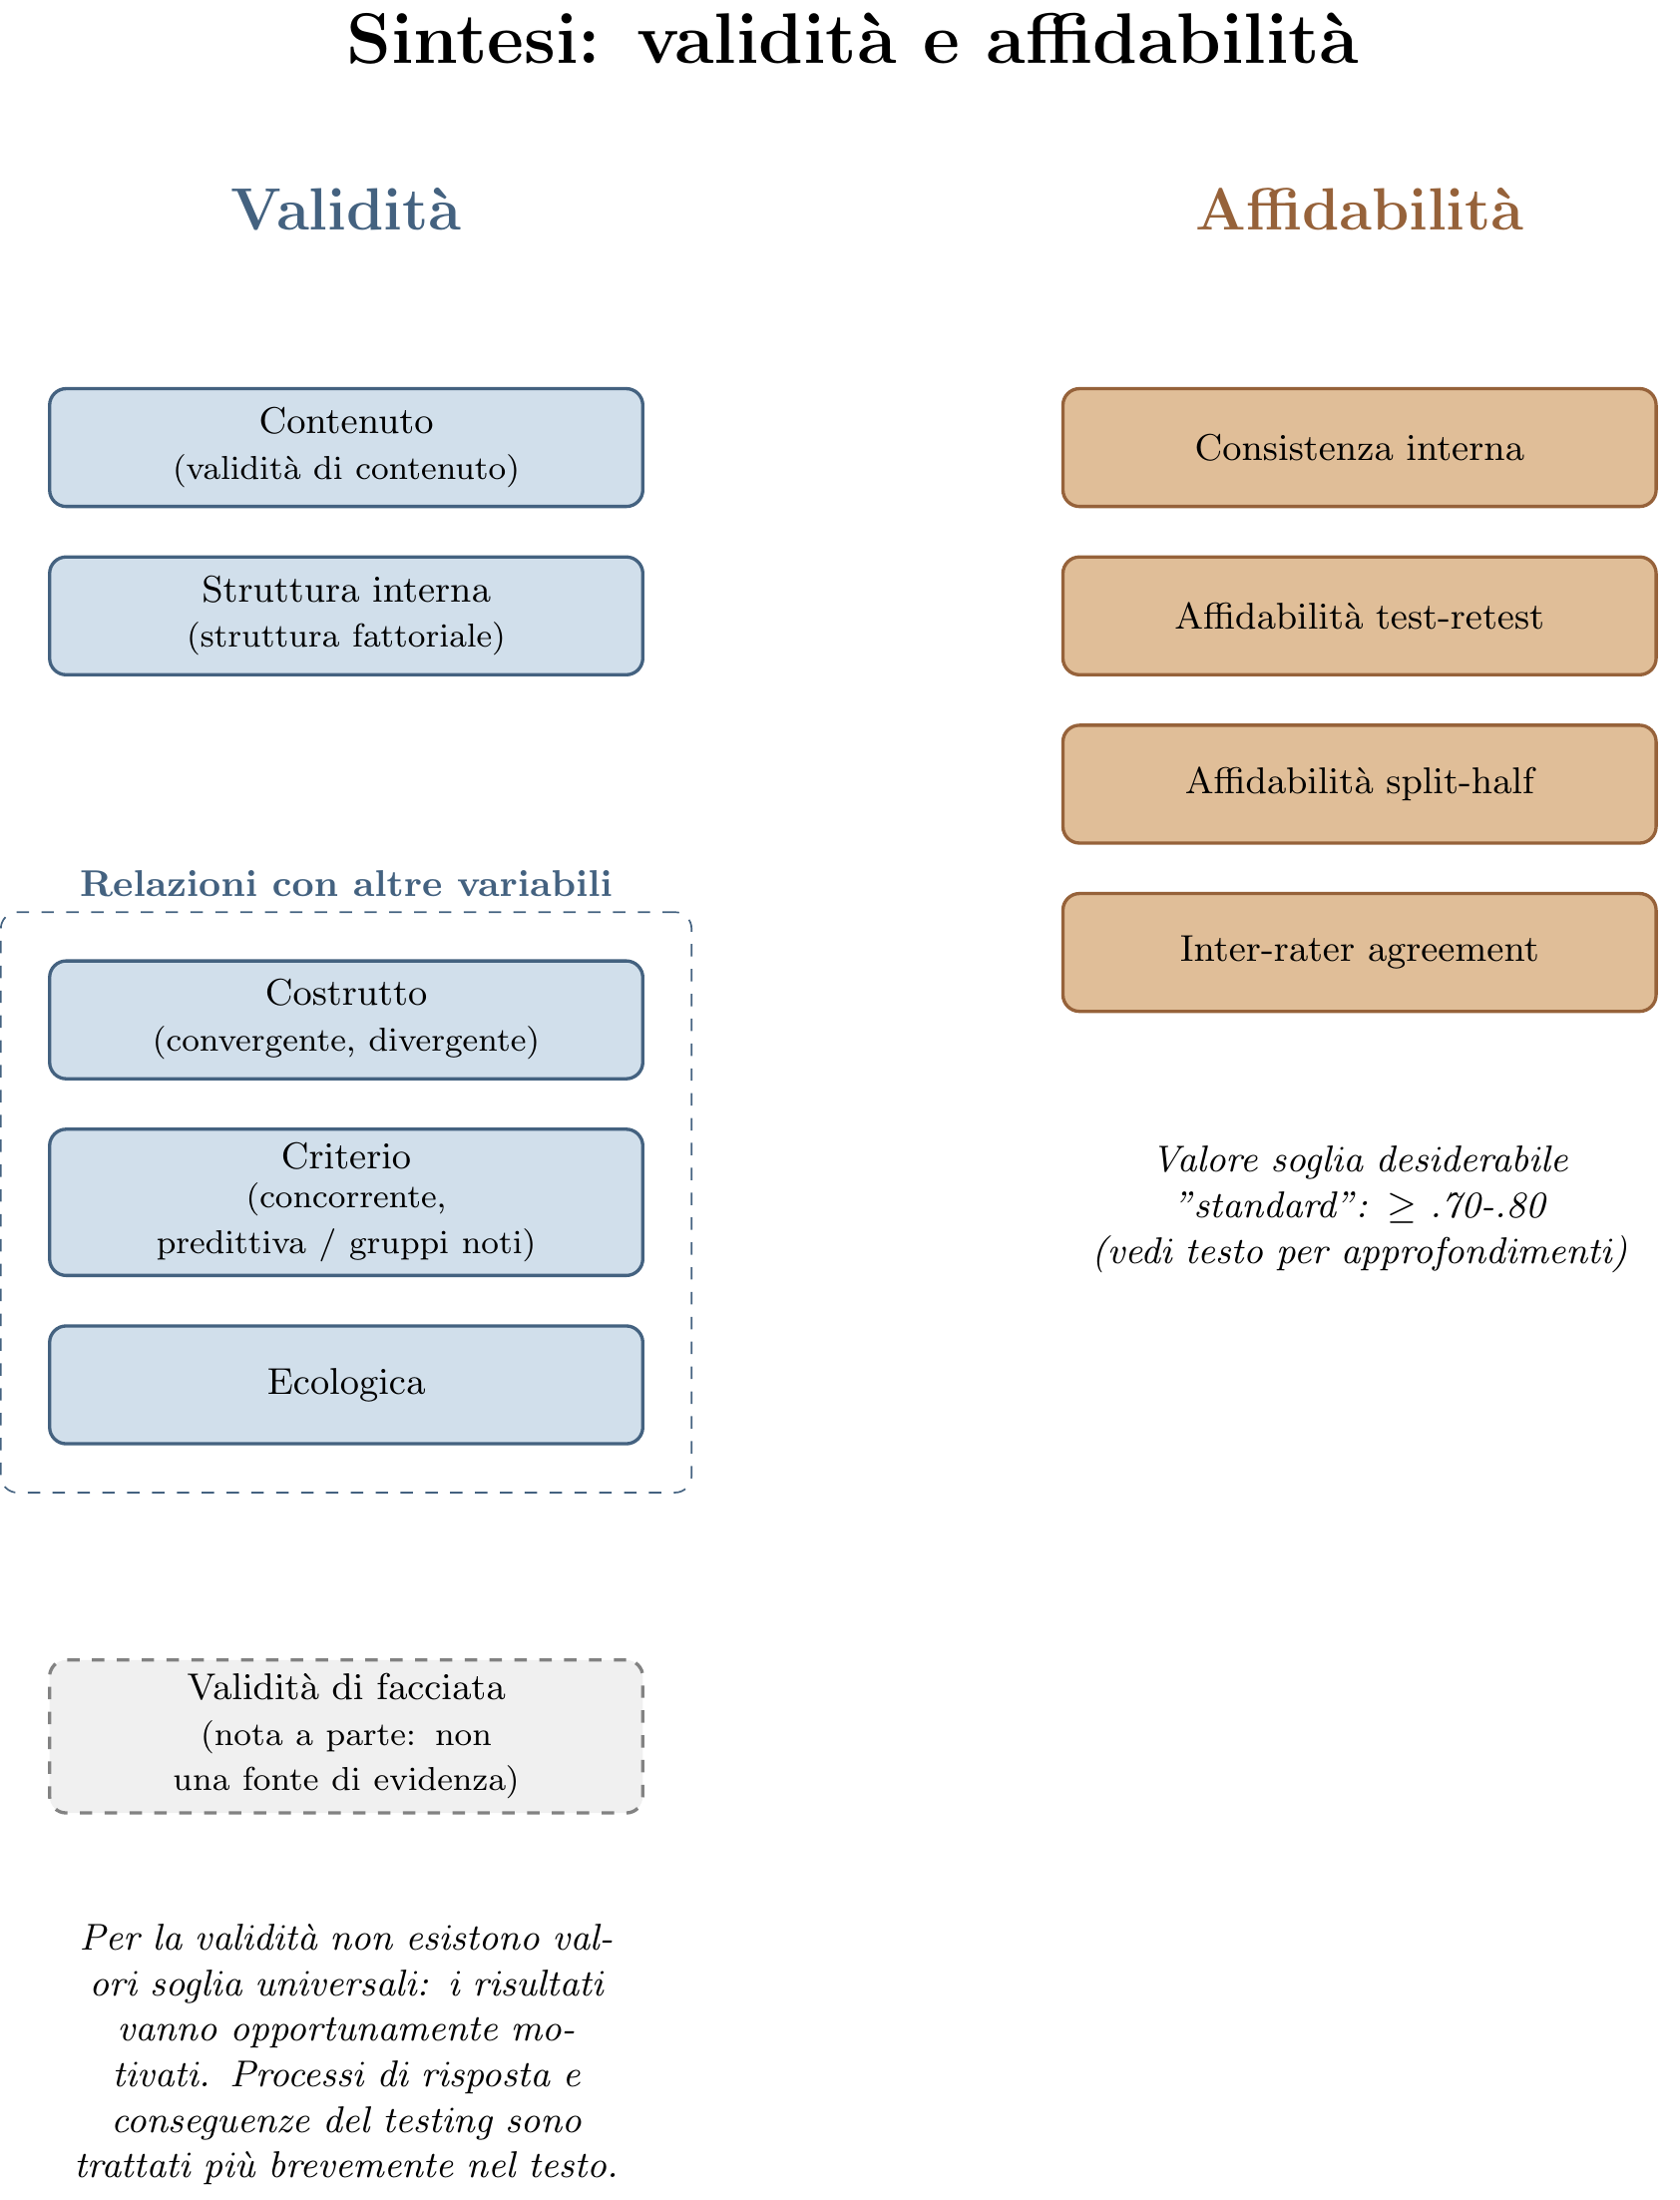
\includegraphics[width=1\linewidth,height=\textheight,keepaspectratio]{chapters/../Figures/Latex-Fig-Validita-Affidabilita/Fig_validita_affidabilita.png}

}

\caption{\label{fig-validita-affidabilita}Sintesi dei tipi di validità e
di affidabilità. A sinistra, i tipi di validità sono raggruppati nelle
due famiglie introdotte all'inizio del capitolo: le validità \textbf{a
priori} (di facciata e di contenuto), valutate sul contenuto del test
prima della raccolta dati, e le validità \textbf{a posteriori} (di
costrutto, di criterio ed ecologica), che richiedono invece evidenze
empiriche. Per la validità non esistono valori soglia universali: i
risultati vanno di volta in volta motivati. A destra, i quattro tipi di
affidabilità trattati nel capitolo, con il valore soglia ``standard''
più diffuso in letteratura (vedi il testo per le soglie più stringenti
raccomandate per le decisioni cliniche sul singolo individuo).}

\end{figure}%

\bookmarksetup{startatroot}

\chapter*{Bibliografia}\label{bibliografia}
\addcontentsline{toc}{chapter}{Bibliografia}

\markboth{Bibliografia}{Bibliografia}

\printbibliography[heading=none]

\bookmarksetup{startatroot}

\chapter*{Lavoro in fase di sviluppo}\label{lavoro-in-fase-di-sviluppo}
\addcontentsline{toc}{chapter}{Lavoro in fase di sviluppo}

\markboth{Lavoro in fase di sviluppo}{Lavoro in fase di sviluppo}

\begin{center}{\Large \textcolor{gray}{\textbf{Questo Libro è ancora in fase di scrittura,\\ per versioni aggiornate visita il sito\\ \url{giorgioarcara.github.io/oip-book} e la newsletter del libro \url{oltreipunteggi.substack.com/}}}} \end{center}

\part{Appendici}

\chapter*{A1. Note di redazione}\label{note_redazione}
\addcontentsline{toc}{chapter}{A1. Note di redazione}

\markboth{A1. Note di redazione}{A1. Note di redazione}

\subsection*{Un libro Open}\label{un-libro-open}
\addcontentsline{toc}{subsection}{Un libro Open}

La decisione di scrivere un libro \emph{Open} (cioè liberamente
scaricabile, modificabile e riutilizzabile) è innanzitutto una scelta
ideologica: sono un convinto sostenitore dell'Open Science da oltre
quindici anni e ritengo che, per un testo di questo tipo, sia l'opzione
più logica. Gran parte dei libri e delle risorse da cui ho appreso i
contenuti che propongo in queste pagine erano, o sono tuttora,
liberamente accessibili, e considero questa modalità non solo sensata,
ma anche eticamente corretta. Oltre alla dimensione ideologica, un libro
\emph{Open} come questo offre ulteriori vantaggi, che verranno
illustrati nel paragrafo seguente.

\subsection*{Un libro collaborativo}\label{un-libro-collaborativo}
\addcontentsline{toc}{subsection}{Un libro collaborativo}

Il libro è pensato per essere scritto anche contando sul contributo dei
lettori. I contributi possono essere segnalazioni di typos, richiesta di
chiarimenti, o di approfondimento, ma sono anche apprezzati anche
commenti generali (es. suggerimenti a rimodulare la struttura di un
capitolo). Non escludo di includere anche intere sezioni scritte da
altre persone, se vorranno contribuire in questa maniera. Ovviamente, se
il contributo sarà sostanziale, la persona sarà inserita tra coautori
del libro. Alla destra di ogni pagina trovi due pulsanti che aiutano per
una comunicazione rapida. Nota che per utilizzarli dovrai però creare un
account \texttt{github}:

\begin{itemize}
\tightlist
\item
  \emph{``Segnala un problema''} può essere utilizzato per segnalare un
  errore generale o se vuoi lasciarmi un commento esteso.
\item
  \emph{``Modifica questa pagina''} , può essere utilizzato se vuoi dare
  un contributo più fattivo e direttamente suggerire una correzione.
  Queste mi verranno segnalato e potrò incorporarle. Puoi utilizzare
  questo strumento per piccole modifiche, ma se pensi di fare una
  modifica sostanziale ti chiedo di contattarmi prima e di concordarla.
  Questo è per rispetto del tuo tempo, nel caso alla fine preferissi non
  inserire la modifica.
\end{itemize}

In alternativa a questi, considera sempre che puoi scrivermi una mail a
\href{mailto:giorgio.arcara@gmail.com}{\nolinkurl{giorgio.arcara@gmail.com}}.
Se sei pratico di github ovviamente sei invitato ad utilizzarlo, creando
una fork e poi aprendo pull request per le modifiche. Ricorda che
contribuendo accetti che i tuoi testi vengano inclusi sotto la licenza
del progetto (CC BY-NC-SA 4.0).

\subsection*{Un libro in costante
miglioramento}\label{un-libro-in-costante-miglioramento}
\addcontentsline{toc}{subsection}{Un libro in costante miglioramento}

Ho scelto di scrivere un libro in questa modalità, tramite un sito e un
.pdf scaricabile associato, perché sono fermamente convinto che (nel
2025, momento in cui sto cominciando a scrivere il volume), bisogna
sfruttare tutte le opportunità date dalla tecnologia. Psicometria e
statistica applicate alla neuropsicologia sono anche discipline in
costante crescita e un libro pubblicato tramite canali tradizionali
rischierebbe di essere obsoleto in alcune sue parti già al momento della
pubblicazione. Usare questo sistema permetterà anche un miglioramento
dopo che il libro potrà essere considerato completo. Il libro usa una
convenzione numerica ispirata al \textbf{Semantic Versioning (SemVer)}
(sistema di numerazione di versioni dei software), adattato al processo
di scrittura.

Il formato è:

\begin{verbatim}
vMAJOR.MINOR.PATCH[-fase]
\end{verbatim}

\subsubsection*{Significato delle parti}\label{significato-delle-parti}
\addcontentsline{toc}{subsubsection}{Significato delle parti}

\begin{itemize}
\tightlist
\item
  \textbf{MAJOR} → Cambia quando viene raggiunta una pietra miliare
  importante (es. bozza completa, revisione principale, versione
  finale).
\item
  \textbf{MINOR} → Cambia quando viene aggiunto un nuovo capitolo o una
  sezione importante, o quando avviene una ristrutturazione
  significativa del testo.
\item
  \textbf{PATCH} → Cambia per correzioni minori, refusi, aggiustamenti
  di frasi, formattazione.
\end{itemize}

\subsubsection*{Etichette di fase}\label{etichette-di-fase}
\addcontentsline{toc}{subsubsection}{Etichette di fase}

\begin{itemize}
\tightlist
\item
  \textbf{alpha} → Bozza iniziale, non revisionata.
\item
  \textbf{beta} → Contenuti quasi completi, pronti per revisione.
\item
  \textbf{rc} (release candidate) → Testo completo e rivisto, in attesa
  di pubblicazione.
\item
  \emph{Nessuna etichetta} → Versione finale.
\end{itemize}

\subsubsection*{Esempi}\label{esempi}
\addcontentsline{toc}{subsubsection}{Esempi}

\begin{verbatim}
v0.1.0-alpha   # Primo capitolo in bozza
v0.1.1-alpha   # Piccole correzioni al primo capitolo
v0.2.0-alpha   # Secondo capitolo in bozza
v1.0.0-beta    # Bozza del libro completa, in revisione
v1.0.0         # Prima Versione finale pubblicata
\end{verbatim}

Nota che la numerazione inizia da \textbf{0} finché il libro non è
completo.

\subsection*{Una nota sul titolo}\label{una-nota-sul-titolo}
\addcontentsline{toc}{subsection}{Una nota sul titolo}

Il titolo del libro, \emph{Oltre i punteggi}, è volto a sottolineare la
mia posizione sull'importanza di integrare i punteggi ai test con altre
informazioni e non penso abbia bisogno di altre spiegazioni. Il
sottitolo del libro invece sottolinea che tratterà di due aspetti,
psicometria e statistica, strettamente legati ma che è utile non
confondere. L'utilizzo dei test neuropsicologici infatti è spesso
(specie in Italia) concentrato molto sulla cura degli aspetti
\emph{statistici} (e in particolare associati a probabilità di ottenere
certi punteggi) ma meno su quelli \emph{psicometrici} e cioè su quanto
accurate sono le nostre misurazioni e su quanto i punteggi che abbiamo
ottenuti siano effettivamente rappresentativi di ciò che ci interessa
(es. il funzionamento cognitivo).

\subsection*{Femminile e maschile nel
testo}\label{femminile-e-maschile-nel-testo}
\addcontentsline{toc}{subsection}{Femminile e maschile nel testo}

In un ottica di gender balance ho deciso di evitare il più possibile di
usare solo il maschile nel testo mettendo ogni volta che fosse
necessario prima femminile e poi maschile (es. la/il neuropsicologa/o).
Questa è una scelta che ho dovuto inevitabilmente fare visto che la
prima stesura del testo è in Italiano. Mi rendo conto che questa scelta,
per quanto motivata, potrebbe rendere più difficile la lettura. Le
evidenze sull'impatto di una scelta come questa nella lettura sono
tuttora non chiare e mi sono basato quindi su un criterio più personale
che non su evidenze scientifiche.

\subsection*{Utilizzo di AI nella stesura del
libro}\label{utilizzo-di-ai-nella-stesura-del-libro}
\addcontentsline{toc}{subsection}{Utilizzo di AI nella stesura del
libro}

Nel momento in cui sto cominciando a scrivere questo libro (Agosto
2025), siamo in piena esplosione dell'utilizzo e delle opportunità di
sistemi di Intelligenza Artificiale (In particolare Large Language
Models, LLM come ChatGPT). Sta diventando sempre più comune dunque
esplicitare che utilizzo se ne è fatto, in maniera trasparente. Tutte le
idee di questo libro sono generate \textbf{senza} l'ausilio di sistemi
di intelligenza artificiale. Sistemi di AI (e in particolare ChatGPT,
Claude, Claude-Code, GitHub Copilot) sono stati utilizzati per i
seguenti scopi:

\begin{itemize}
\tightlist
\item
  revisione del testo (per typos o miglioramento chiarezza di alcune
  frasi)
\item
  supporto nel codice per generare il libro (Quarto e i linguaggi
  associati).
\item
  generazioni di alcune immagini esemplificative o per l'immagine di
  copertina (questo per evitare problemi di immagini con copyright).
\item
  supporto nella generazione di codice \texttt{R} per alcuni esempi.
\item
  ricerca di letteratura (citazioni per le quali non è stato possibile
  verificare la fonte originale, non sono mai riportate).
\end{itemize}

In ogni caso, mi prendo ogni responsabilità di errori legati
all'utilizzo di sistemi di AI.

\chapter*{A2. Registro aggiornamenti}\label{registro_aggiornamenti}
\addcontentsline{toc}{chapter}{A2. Registro aggiornamenti}

\markboth{A2. Registro aggiornamenti}{A2. Registro aggiornamenti}

\subsection*{v0.0.1 - 5/09/2025}\label{v0.0.1---5092025}
\addcontentsline{toc}{subsection}{v0.0.1 - 5/09/2025}

Rilasciata versione iniziale del libro che include

\begin{itemize}
\tightlist
\item
  Premesse
\item
  Introduzione
\item
  Appendici A1 e A2
\end{itemize}

\subsection*{v0.1.0}\label{v0.1.0}
\addcontentsline{toc}{subsection}{v0.1.0}

\begin{itemize}
\tightlist
\item
  corretti vari typos e migliorato il flusso di alcune frasi.
\item
  aggiunta quarta di copertina.
\item
  aggiunta prima versione del Capitolo 1.
\item
  aggiunta previsione di nuovi paragrafi (Riassunti a fine capitolo e
  paragrafo su AI).
\end{itemize}

\subsection*{v0.1.1}\label{v0.1.1}
\addcontentsline{toc}{subsection}{v0.1.1}

\begin{itemize}
\tightlist
\item
  aggiunta prima parte paragrafo misurazione
\end{itemize}

\subsection*{v0.1.2}\label{v0.1.2}
\addcontentsline{toc}{subsection}{v0.1.2}

\begin{itemize}
\tightlist
\item
  migliorata prima parte paragrafo misurazione.
\end{itemize}

\subsection*{v0.1.3}\label{v0.1.3}
\addcontentsline{toc}{subsection}{v0.1.3}

\begin{itemize}
\tightlist
\item
  aggiunta sezione su Validità (teoria).
\item
  aggiornata figura sulla CTT.
\item
  aggiornata sezione su Validità.
\end{itemize}

\subsection*{v0.2.0}\label{v0.2.0}
\addcontentsline{toc}{subsection}{v0.2.0}

\begin{itemize}
\tightlist
\item
  separata la sezione Validità e Affidabilità in un capitolo autonomo
  (chapters/Validita-Affidabilita.qmd), distinto dal capitolo su
  misurazione e test (rinominato ``Misurazione e Test in Neuropsicologia
  Clinica'').
\item
  aggiornati indice provvisorio e riferimenti incrociati (Introduzione,
  numerazione dei capitoli) di conseguenza.
\end{itemize}

\subsection*{v0.2.1}\label{v0.2.1}
\addcontentsline{toc}{subsection}{v0.2.1}

\begin{itemize}
\tightlist
\item
  corrette numerose citazioni non inserite correttamente nello standard
  a doppio rendering (LaTeX/HTML): parentesi sbilanciate, citazioni
  narrative con nome autore duplicato, citazioni testuali senza markup.
\item
  aggiunte citazioni a references.bib.
\end{itemize}

\chapter*{A3. Definizioni}\label{definizioni}
\addcontentsline{toc}{chapter}{A3. Definizioni}

\markboth{A3. Definizioni}{A3. Definizioni}

\subsection*{Perché sono importanti le
definizioni.}\label{perchuxe9-sono-importanti-le-definizioni.}
\addcontentsline{toc}{subsection}{Perché sono importanti le
definizioni.}

Un libro che ambisce a insegnare l'importanza della metodologia non può
prescindere dall'includere una sezione con le definizioni dei termini
più importanti. Wittgenstein in una delle più famose proposizioni del
suo \emph{Tractatus} affermava:

\emph{5.6 I limiti del mio linguaggio sono i limiti del mio mondo.}

Senza scendere nel dettaglio delle implicazioni di questa asserzione, è
utile riflettere sul fatto che il modo in cui definiamo le entità che ci
interessano definiscono il confine entro cui ci muoviamo e, anche se ce
ne rendiamo conto, influenzano in maniera determinante la metodologia e
il nostro approccio alla clinica. Si pensi a parole che usiamo
frequentemente nella pratica clinica, come \emph{deficit},
\emph{normalità}, \emph{peggioramento}. L'esatta sfumatura che diamo a
questi significati ha un grande impatto sulla nostra pratica clinica e,
per quanto riguarda la metodologia, nello stabilire se un metodo è
adeguato oppure no.

\subsubsection*{Psicometria}\label{psicometria}
\addcontentsline{toc}{subsubsection}{Psicometria}

La Psicometria è quella disciplina che studia teorie e metodi di
misurazione in psicologia. Nello specifico si occupa di test,
misurazioni e valutazioni di tipo psicologico e di misurazione di
costrutti latenti, cioè non osservabili.
(\href{https://en.wikipedia.org/w/index.php?title=Psychometrics&oldid=1307897603}{(fonte:
Wikpedia)}

\emph{Nota}: la psicometria fa grande utilizzo di metodi di statistica,
tanto che, specie in ambito psicologico, spesso c'è confusione tra i
confini tra le due discipline. Anche se è vero che ci sono numerose aree
di sovrapposizione (perché la Psicometria fa utilizzo di tecniche
statistiche), non sono da considerare come sinonimi, visto che molti
aspetti psicometrici non sono strettamente statistici e numerosi aspetti
statistici non è detto che siano rilevanti per la psicometria.

\subsubsection*{Statistica}\label{statistica}
\addcontentsline{toc}{subsubsection}{Statistica}

La statistica è quella disciplina che studia la raccolta, descrizione,
analisi e interpretazione di \emph{dati}, La statistica si occupa di
ogni fase del trattamento dei dati, dalla pianificazione dei disegni,
fino alle tecniche di analisi e inferenze sui risultati ottenuti.
\href{https://en.wikipedia.org/w/index.php?title=Statistics&oldid=1307451692}{(fonte:
Wikpedia)}

\emph{Nota}: è importante conoscere la statistica non solo perché essa
viene utilizzata abbondantemente in psicometria, ma anche perché certi
aspetti rilevanti per le interpretazioni di test neuropsicologici sono
meramente statistici (e non psicometrici, secondo la definizione di
``psicometria'' riportata sopra). Ad esempio stimare le probabilità di
classificare un paziente come a rischio di Alzheimer a partire da dati
biologici e anamnestici non prevede misurazioni di costrutti psicologici
e quindi non è pertinenza delle psicometria.

\subsubsection*{Valutazione
neuropsicologica}\label{valutazione-neuropsicologica}
\addcontentsline{toc}{subsubsection}{Valutazione neuropsicologica}

La valutazione neuropsicologica è un esame clinico in cui si cerca di
ottenere informazioni sullo stato cognitivo di un individuo a fini
diagnostici, prognostici o riabilitativi. Essa consiste in genere in
raccolta di dati anamnestici, un colloquio e la somministrazione di test
standardizzati. Tutte queste informazioni sono integrate per stilare un
referto neuropsicologico.

\subsubsection*{Costrutto}\label{costrutto}
\addcontentsline{toc}{subsubsection}{Costrutto}

Un concetto psicologico non direttamente osservabile. Sono esempi di
costrutti, esempi come Ansia, Depressione, Memoria, Attenzione, etc. I
costrutti sono osservabili tramite \emph{comportamenti} direttamente
osservabili che si assume siano associati al costrutto. Un aspetto
fondamentale (e caratteristico della Psicometria) è che la relazione tra
Costrutto e comportamenti osservabili non è mai perfetta.

\chapter*{Ringraziamenti personali}\label{ringraziamenti_personali}
\addcontentsline{toc}{chapter}{Ringraziamenti personali}

\markboth{Ringraziamenti personali}{Ringraziamenti personali}

Tutti i ringraziamenti che seguono vanno considerati in ordine sparso,
senza una gerarchia particolare.

Ringrazio la mia supervisor di dottorato, la Prof.ssa Sara Mondini, per
avermi fatto appassionare alla neuropsicologia clinica e per le numerose
interessantissime discussioni. Diverse parti di questo libro sono state
sviluppate a partire da scambi con lei e sono almeno in parte state già
riportate in altri testi, che abbiamo scritto anche insieme alla
Prof.ssa Daniela Mapelli e la Prof.ssa Marinella Cappelletti.

Ringrazio il Prof.~Carlo Semenza, per avermi fatto sempre credere
nell'importanza di porsi domande, anche quando sembrano controcorrente,
e per avermi trasmesso la passione alla neuropsicologia e alla scienza.

Ringrazio tutto il personale clinico con cui ho avuto modo di discutere
e collaborare in questi anni. Molto di quanto scritto riflette delle
discussioni fatte con loro e il tentativo di rispondere a domande che mi
sono state poste proprio da loro.

Vorrei ringraziare i membri del Quantitative Psychology Lab (QP Lab),
del Dipartimento di Psicologia Generale dell'Università di Padova per le
discussioni stimolanti e le considerazioni. Varie parti di questo libro
sono state sviluppate a partire da scambi con loro, spesso illuminanti.
In ordine alfabetico: Giovanni Bruno, Umberto Granziol, Stefano Noventa,
Massimo Nucci, Andrea Spoto, Michele Vicovaro.

Grazie a Rachele, per la sua pazienza senza fine.


\backmatter


\end{document}
